%%%%%%%%%%%%%%%%%%%%%%%%%%%%%%%%%%%%%%%%%%%%%%%%%%%%%%%%%%%%%%%%%%%%%%
%% SignalShap -- manuscript draft for Discover Artificial Intelligence
%% Springer Nature journal template (sn-jnl.cls, v3.1 December 2024)
%%
%% Compile: pdflatex -> bibtex -> pdflatex -> pdflatex
%% Requires: sn-jnl.cls and sn-mathphys-num.bst in the same directory,
%%           plus signalshap-bibliography.bib
%%
%% STRUCTURE
%%   Six-section layout of the authors' IJACSA 2025 paper [louhichi2025]:
%%     1 Introduction (flat, numbered contributions list, roadmap)
%%     2 Literature review (thematic subsections, each closing on a gap)
%%     3 Methodology (pipeline subsections; comparative analysis,
%%       theoretical justification, complexity, and practical
%%       implementation as the closing subsections)
%%     4 Experimental results (setup and results combined)
%%     5 Discussion and broader implications
%%     6 Conclusion
%%   Declarations and appendices are retained: declarations are mandatory
%%   for Springer, and the proofs need somewhere to live.
%%
%% CONVENTIONS USED IN THIS DRAFT
%%   SELF-CONTAINED SUBMISSION FOLDER. Everything needed to typeset this
%%   manuscript lives beside this file:
%%     signalshap.tex              this file
%%     signalshap-bibliography.bib 46 references, all cited
%%     sn-jnl.cls                  Springer Nature class
%%     sn-mathphys-num.bst         Springer Nature numeric bib style
%%     tables/                     generated table bodies + numeric macros
%%     figures/                    result figures (PNG)
%%
%%   Compile: pdflatex -> bibtex -> pdflatex -> pdflatex
%%
%%   ALL RESULTS IN THIS MANUSCRIPT ARE REAL. Every numeric value is
%%   generated from the experiment output (code/results/raw/*.json in the
%%   source repository) by code/scripts/emit_paper_tables.py, which writes
%%   the fragments in tables/ that are \input below. No number is
%%   transcribed by hand; see README.md in this folder to regenerate.
%%
%%   Figure 1 (architecture) and Figure 5 (segment correspondence) are the
%%   only two still drawn as placeholder boxes; both are schematics rather
%%   than result plots.
%%
%% CALIBRATION
%%   Theory is deliberately light -- three short propositions and one
%%   remark -- to match the level of [nesmaoui2026drift], which carries
%%   no propositions at all. Do not add more.
%%%%%%%%%%%%%%%%%%%%%%%%%%%%%%%%%%%%%%%%%%%%%%%%%%%%%%%%%%%%%%%%%%%%%%

\documentclass[pdflatex,sn-mathphys-num]{sn-jnl}% Math and Physical Sciences Numbered Reference Style

%%%% Standard packages (as shipped with the template)
\usepackage{graphicx}%
\graphicspath{{figures/}}%
\newcommand{\resdir}{tables}%
\usepackage{multirow}%
\usepackage{amsmath,amssymb,amsfonts}%
\usepackage{amsthm}%
\usepackage{mathrsfs}%
\usepackage[title]{appendix}%
\usepackage{xcolor}%
\usepackage{textcomp}%
\usepackage{manyfoot}%
\usepackage{booktabs}%
%% Package list follows the official Springer sn-jnl template exactly.
%% algorithmicx and algpseudocode are BOTH loaded there; that combination is
%% supported and is what supplies \State, \Require, \For, \If, \Comment.
\usepackage{algorithm}%
\usepackage{algorithmicx}%
\usepackage{algpseudocode}%
%% TikZ for the architecture diagram (Figure 1). Drawn natively so the figure
%% is vector, editable, and needs no external image file.
\usepackage{tikz}%
\usetikzlibrary{shapes.geometric,arrows.meta,positioning,fit,calc}%
%% NOTE: the float package is deliberately NOT loaded. It is absent from the
%% official Springer template and its [H] specifier interacts badly with the
%% algorithm package's own float registration. Appendix B tables use [t]
%% instead; they are long, so letting LaTeX place them is correct anyway.
%% sn-jnl.cls already loads hyperref (which provides \url) and breakurl, so
%% the url package is deliberately NOT loaded.

%%%% Theorem-like environments
\theoremstyle{thmstyleone}%
\newtheorem{theorem}{Theorem}%
\newtheorem{proposition}[theorem]{Proposition}%
\newtheorem{corollary}[theorem]{Corollary}%

\theoremstyle{thmstyletwo}%
\newtheorem{example}{Example}%
\newtheorem{remark}{Remark}%

\theoremstyle{thmstylethree}%
\newtheorem{definition}{Definition}%

%%%% Draft-only macros. Remove both before submission.
%% Numeric macros generated from the result JSONs -- do not edit by hand.
%% If this file is missing every \recMl-style value becomes an undefined
%% control sequence, so fail loudly and early instead.
\IfFileExists{tables/macros.tex}{%
  \input{tables/macros.tex}%
}{%
  \ClassError{sn-jnl}{Missing tables/macros.tex -- run 'make refresh'}{%
  Every numeric value in this manuscript is generated. See README.md.}%
}
%% \tbd is retained only for genuinely open editorial items; none remain
%% in the results sections.
\newcommand{\tbd}[1]{\textbf{[#1]}}
%% (\figph placeholder macro removed: no placeholders remain)

%%%% Shorthands
\newcommand{\NDCG}{\mathrm{NDCG@10}}
\newcommand{\LOO}{\mathrm{LOO}}
\newcommand{\Gset}{\mathcal{G}}
\newcommand{\Uset}{\mathcal{U}}
\newcommand{\Iset}{\mathcal{I}}

\raggedbottom

\begin{document}

\title[Exact Fusion-Stage Shapley Attribution]{Exact Fusion-Stage Shapley Attribution over the Signal Sources of a Hybrid Recommender}

\author*[1]{\fnm{Mouad} \sur{Louhichi}}\email{mouad\_louhichi@um5.ac.ma}

\author[1]{\fnm{Redwane} \sur{Nesmaoui}}\email{redwane\_nesmaoui@um5.ac.ma}

\author[1]{\fnm{Mohamed} \sur{Lazaar}}\email{mohamed.lazaar@ensias.um5.ac.ma}

\affil*[1]{\orgdiv{National Higher School of Computer Science and Systems Analysis (ENSIAS)}, \orgname{Mohammed V University in Rabat}, \orgaddress{\city{Rabat}, \country{Morocco}}}

%%==================================%%
%% Abstract: Discover AI asks for 150--250 words, unstructured,
%% no citations, no equations. Current length ~215 words.
%%==================================%%

\abstract{Hybrid recommender systems combine collaborative, content, popularity, temporal, and sequential signals into a single ranking, yet practitioners have no principled account of which source earns the resulting accuracy. We answer that question at the fusion stage, holding the retrieval pool fixed across coalitions so that sources are compared on a common candidate set. The prevailing answer, which is to remove one source and measure the drop, is misleading whenever sources are redundant, a condition that is the norm rather than the exception in recommendation, because two mutually substitutable sources each receive zero credit. We recast hybrid recommendation as a cooperative game in which the players are the signal sources and the characteristic function is ranking quality, and we compute the exact Shapley allocation. The player set is small by construction, so no sampling approximation is required, and because the base scorers are trained once while only a lightweight fusion layer is refitted per coalition, the full game runs in under a minute on a laptop CPU. We show that efficiency yields an exact additive decomposition of ranking-quality uplift, that leave-one-out collapses to zero under perfect redundancy where the Shapley value splits credit evenly, and that linearity makes per-user attribution available with no additional coalition refits. Aggregating per-user attributions into behavioural segments shows that global source credit conceals opposing segment-level stories. Exploiting this, segment-adaptive fusion weights improve ranking quality over a globally tuned hybrid at no additional inference cost on one of the three benchmarks, with no significant change on the other two. Experiments span one dense and two sparse benchmarks: MovieLens-1M, Amazon-Beauty, and Amazon-Grocery. Against SASRec and LightGCN, both trained and evaluated inside the same pipeline, the hybrid is statistically indistinguishable from SASRec on the dense benchmark, roughly forty percent ahead of SASRec on both sparse ones, and ahead of LightGCN on all three, so the allocation describes a system that is competitive against the two controlled references evaluated here. Because every coalition is scored on a candidate pool built by the full source set, the allocation measures fusion-stage credit rather than the end-to-end value of operating a source, and we quantify the gap between the two directly: on a matched seed, regenerating the pool per coalition shifts no source's share by more than \regenworst\ percentage points and preserves the ordering on every benchmark. With six sources the game has $2^{6}=64$ coalitions and the complete sweep runs in under a minute on a laptop CPU, with the efficiency identity holding to machine precision. Leave-one-out recovers only \looshMlc\%, \looshBtc\% and \looshGrc\% of the uplift it purports to explain on the three datasets; in the sharpest case it reports the second-strongest collaborative source as actively harmful ($\looMlEASE$) where the Shapley value assigns it \shMlEASE\% of all ranking-quality gain. We also report what did not hold: of four pre-registered predictions the data contradicted one, we withdrew a second, a third held on one benchmark of three, and a fourth proved partly an artifact of temporal resolution.}

%% Discover AI requests 3--6 keywords.
\keywords{Shapley value, Cooperative game theory, Explainable AI, Recommender systems, Credit assignment, User segmentation}

\maketitle

%%%%%%%%%%%%%%%%%%%%%%%%%%%%%%%%%%%%%%%%%%%%%%%%%%%%%%%%%%%%%%%%%%%%%%
\section{Introduction}\label{sec1}
%%%%%%%%%%%%%%%%%%%%%%%%%%%%%%%%%%%%%%%%%%%%%%%%%%%%%%%%%%%%%%%%%%%%%%
%% Flat, no subheadings: required by the Springer template and matching
%% the introductions of [louhichi2023, louhichi2025, louhichi2026].
%% Closes with a numbered contributions list and a roadmap paragraph.

Deployed recommender systems are almost never a single model. They are hybrids that combine a collaborative signal learned from interaction co-occurrence, a content signal derived from item metadata, a popularity prior, a temporal or recency signal, and a sequential signal that conditions on what the user did last \cite{burke2002}. Each of these arrives through its own pipeline and each carries its own running cost. A content signal requires metadata ingestion, cleaning, and reconciliation across catalogue updates. A sequential model requires session logging and low-latency access to recent state. A collaborative model requires an interaction store and periodic retraining. A team maintaining five such pipelines operates under a fixed engineering budget and must decide which of them deserves that budget, yet has no defensible basis on which to decide, because the accuracy of the hybrid is reported as a single number that no one knows how to divide.

This is a question about credit, and it is not the question that explainable recommendation has been answering. That literature has concentrated, with considerable success, on explaining \emph{why a particular item was shown to a particular user}: item-level justifications, knowledge-graph paths, counterfactual statements, and review-derived rationales, all aimed at the end user who receives the recommendation \cite{zhang2020}. The audience we address is different. It is the system owner, who does not ask why an item appeared but rather \emph{which part of my system is producing the value I am paying for}. That audience is essentially unserved, and the gap is easy to state: existing explanation targets are items and features, whereas the object the system owner reasons about is the signal source.

The obvious way to answer the question is ablation. Remove one source, retrain or refit, and measure how far ranking quality falls. This is standard practice and it is wrong in a way that matters specifically in recommendation. Suppose the content signal and the collaborative signal happen to rank the same items highly for a given user. Deleting either one alone changes almost nothing, because the other continues to supply the same ordering, so ablation reports that \emph{neither source matters}. Deleting both is catastrophic. Leave-one-out therefore assigns near-zero credit to sources that are jointly load-bearing, and the sum of its verdicts bears no particular relation to the total quality it is trying to explain. Redundancy of exactly this kind is the norm in recommendation rather than the exception: popularity signals leak into collaborative embeddings \cite{abdollahpouri2019,cremonesi2010}, content and collaborative signals converge on the same catalogue neighbourhoods, and static and time-weighted popularity are two views of one underlying quantity. Proposition~\ref{prop2} makes this failure precise.

Cooperative game theory supplies the correction, and supplies it with axioms rather than heuristics. The Shapley value \cite{shapley1953} allocates credit so that the allocation is efficient, symmetric, additive, and assigns nothing to a null player; efficiency in particular guarantees that the shares sum exactly to the quantity being explained, which is the property ablation lacks. These axioms characterize the allocation uniquely, and an alternative characterization via strong monotonicity \cite{young1985monotonic} makes the same point in a form that is arguably closer to the intuition a system owner brings: a source whose marginal contributions never decrease cannot see its credit fall. The Shapley value has become the dominant formal instrument in explainable machine learning through SHAP and its descendants \cite{lundberg2017,lundberg2020,covert2021,li2024shapley}, and it underpins the present authors' prior work on explaining clustering \cite{louhichi2023,louhichi2025} and on cooperative allocation in recommendation \cite{louhichi2026,nesmaoui2025}.

The standing objection to Shapley-based explanation is cost. Exact computation requires evaluating $2^{n}$ coalitions, which is why the literature has invested so heavily in sampling estimators \cite{castro2009,strumbelj2010} and why prior work routinely adopts Monte-Carlo approximation. We observe that this objection is not a property of the Shapley value but of the choice to make \emph{features} the players. When the players are \emph{signal sources}, the player set is small by construction: a hybrid with six sources induces sixty-four coalitions. Combined with an architecture in which base scorers are trained once and only a lightweight fusion layer is refitted per coalition, the exact allocation becomes not merely tractable but cheap, and indeed cheaper, as Section~\ref{subsec3_10} shows, than training the recommender it explains. The contributions are as follows.

\begin{enumerate}
\item \textbf{A cooperative game over signal sources.} We formalize hybrid recommendation as a transferable-utility game whose players are signal sources rather than features or items, and whose characteristic function is ranking quality measured against a null ranker. Because the player set is small by construction, the Shapley allocation is computed exactly, with no Monte-Carlo estimation and no approximation error to bound.

\item \textbf{Three short results that make the allocation usable.} Efficiency yields an exact additive decomposition of ranking-quality uplift into per-source shares (Proposition~\ref{prop1}). Under perfect redundancy, leave-one-out assigns zero to both members of a redundant pair while the Shapley value splits the credit evenly, which identifies formally the failure mode motivating this work (Proposition~\ref{prop2}). Linearity of the Shapley operator over a per-user-mean characteristic function makes per-user attribution available at no computational cost beyond the global game (Proposition~\ref{prop3}).

\item \textbf{Segment-level source profiles.} Aggregating per-user attributions over behavioural segments shows that global source credit is an average over heterogeneous and sometimes opposing populations. We quantify the heterogeneity with a permutation test and identify the segments in which the global ordering inverts.

\item \textbf{Segment-adaptive fusion, with a qualified outcome.} We use the segment profiles to set per-segment fusion weights, converting an explanation into a candidate intervention at no additional inference cost, since segment assignment is a table lookup. The result is mixed and we present it as such: a significant \gainGr\% improvement on one benchmark and no significant change on the other two, which is weaker than we had predicted and is reported without reframing.

\item \textbf{A reproducibility-oriented report.} All six sources are standard published methods with public implementations, base scorers are trained once and cached, and the entire game runs on a laptop CPU. Every hyperparameter, seed, and preprocessing decision is tabulated in the paper, and the full coalition values are given in Appendix~\ref{secA2} so that the allocation can be recomputed independently of our code.
\end{enumerate}

The remainder of the paper is organized as follows. Section~\ref{sec2} reviews hybrid recommendation, explainable recommendation, Shapley-based attribution, cooperative games over model components, and heterogeneous explanation, closing with a positioning table. Section~\ref{sec3} presents the source-attribution game, the fusion architecture that makes it cheap, the per-user and per-segment decomposition, segment-adaptive fusion, the theoretical justification, and a complexity analysis. Section~\ref{sec4} reports the experimental protocol and results against four research questions. Section~\ref{sec5} discusses what the attributions imply for system design, and Section~\ref{sec6} concludes.

%%%%%%%%%%%%%%%%%%%%%%%%%%%%%%%%%%%%%%%%%%%%%%%%%%%%%%%%%%%%%%%%%%%%%%
\section{Literature review}\label{sec2}
%%%%%%%%%%%%%%%%%%%%%%%%%%%%%%%%%%%%%%%%%%%%%%%%%%%%%%%%%%%%%%%%%%%%%%
%% Thematic subsections, each closing on an explicit gap sentence,
%% following the pattern of [louhichi2025] and [nesmaoui2026drift].

\subsection{Hybrid recommendation and score-level fusion}\label{subsec2_1}

Burke's taxonomy of hybridization \cite{burke2002} distinguishes weighted, switching, cascade, feature-combination, and meta-level designs. Of these, the weighted or score-level pattern, in which each component produces a score and a fusion stage combines them, has become the dominant production architecture, in part because it decouples component development from combination logic and in part because it composes naturally with the two-stage retrieval-then-ranking pipelines used at scale \cite{covington2016}. The components themselves are well studied in isolation: matrix factorization and its implicit-feedback variants \cite{koren2009,rendle2009}, content-based similarity over item descriptors \cite{salton1988}, popularity baselines whose competitiveness on top-$N$ tasks is a recurring finding \cite{cremonesi2010}, and sequential models from Markov chains \cite{rendle2010} to self-attention \cite{kang2018}.

Score-level fusion is also the pattern that makes source-level ablation well defined, since a source can be withheld from the combination without redesigning the architecture, and this is why we adopt it. \emph{The gap: this literature optimizes fusion weights extensively but never asks what each fused source contributes to the result.}

\subsection{Explainability in recommender systems}\label{subsec2_2}

Explainable recommendation is a mature field with its own survey literature \cite{zhang2020}. Its methods generate post-hoc item-level justifications, trace paths through knowledge graphs, produce counterfactual statements about what would have changed a recommendation, or surface review text as evidence. What unites them is the audience: all are addressed to the end user, and all take an individual recommendation as the unit of explanation.

\emph{The gap: the system-owner audience, whose unit of explanation is the architectural component rather than the recommended item, is not addressed.}

\subsection{Shapley values in machine learning and explainable AI}\label{subsec2_3}

The Shapley value \cite{shapley1953} entered machine learning as a principled answer to feature attribution, formalized in the SHAP family \cite{lundberg2017} and extended to tractable model classes \cite{lundberg2020} and to a general removal-based framework \cite{covert2021} that also subsumes earlier surrogate-based explainers such as LIME \cite{ribeiro2016}. Recent surveys consolidate its axiomatic appeal and catalogue its practical limitations \cite{li2024shapley}. The dominant limitation is computational: exact evaluation is exponential in the number of players, which has motivated a substantial line of sampling estimators \cite{castro2009,strumbelj2010}.

The authors' prior work sits on both sides of this trade-off. Feature-level Shapley attribution over clustering surrogates \cite{louhichi2023,louhichi2025} accepts the feature player set and the approximation it entails, while work on temporal explanation stability adopts Monte-Carlo estimation explicitly because exact computation over features is infeasible.

\emph{The gap: the computational objection is treated as intrinsic to the Shapley value, when it is a consequence of the choice of player set.}

\subsection{Cooperative games over components, data, and features}\label{subsec2_4}

A parallel line of work replaces features with other players. Data Shapley values individual training points \cite{ghorbani2019}. Structured player sets are handled by the Owen value when players form a priori unions \cite{owen1977} and by the Myerson value when cooperation is restricted by a graph \cite{myerson1977}; the authors have applied graph- and hypergraph-restricted allocation to preference modelling \cite{louhichi2026} and to real-time contribution adjustment in dynamic recommenders \cite{nesmaoui2025}.

\emph{The gap: the signal source is a natural player set for hybrid systems, and it has not been instantiated.}

\subsection{User segmentation and heterogeneous explanation}\label{subsec2_5}

Clustering has long been used to model user populations, and it is well recognized that a global explanation is an average over a population that may not be homogeneous. The authors' clustering-plus-Shapley line \cite{louhichi2023,louhichi2025} establishes the precedent for treating segments as the explanatory unit rather than as a preprocessing step.

\emph{The gap: population heterogeneity in attribution has not been measured for architectural components, nor exploited to improve the system.}

\subsection{Positioning}\label{subsec2_6}

Table~\ref{tab1} places this work against representative alternatives along four axes: the unit to which credit is assigned, whether the allocation carries an axiomatic guarantee, whether it is exact or approximate, whether it is heterogeneity-aware, and whether it closes the loop from explanation back to system improvement.

\begin{table}[t]
\caption{Positioning against representative prior work. ``Loop'' indicates whether the attribution is fed back to improve the system.}\label{tab1}
\small
\setlength{\tabcolsep}{4pt}
\begin{tabular}{@{}p{0.30\linewidth}p{0.13\linewidth}ccp{0.12\linewidth}c@{}}
\toprule
Method family & Unit & Axiom. & Exact & Heterog. & Loop \\
\midrule
Item-level explainable rec.\ \cite{zhang2020} & item & no & n/a & no & no \\
Feature SHAP \cite{lundberg2017,lundberg2020} & feature & yes & no & no & no \\
Data Shapley \cite{ghorbani2019} & datum & yes & no & no & partial \\
Clustering + Shapley \cite{louhichi2023,louhichi2025} & feature & yes & no & partial & no \\
Cooperative rec.\ \cite{louhichi2026,nesmaoui2025} & node/edge & yes & no & no & yes \\
Ablation / leave-one-out & source & no & yes & no & no \\
\textbf{SignalShap (this work)} & \textbf{source} & \textbf{yes} & \textbf{yes} & \textbf{yes} & \textbf{yes} \\
\bottomrule
\end{tabular}
\end{table}

%%%%%%%%%%%%%%%%%%%%%%%%%%%%%%%%%%%%%%%%%%%%%%%%%%%%%%%%%%%%%%%%%%%%%%
\section{Background}\label{sec2b}

This section fixes the cooperative-game vocabulary used throughout. Readers
familiar with the Shapley value may skip to Section~\ref{sec3}.

\paragraph{Transferable-utility games.}
A cooperative game with transferable utility is a pair $(\Gset, v)$ where
$\Gset$ is a finite set of $K$ players and $v:2^{\Gset}\to\mathbb{R}$ is a
characteristic function with $v(\emptyset)=0$. The quantity $v(C)$ is the
worth that coalition $C$ can secure on its own. In our setting the players are
signal sources and $v(C)$ is the ranking quality attained by a hybrid built
from exactly those sources; transferability is the assumption that this worth
is a single real number that can be divided among the sources, which holds
because NDCG@10 is a scalar.

\paragraph{The Shapley value and its axioms.}
An allocation rule assigns each player $g$ a share $\varphi_g$ of $v(\Gset)$.
The Shapley value \cite{shapley1953} is the unique rule satisfying four
axioms. \emph{Efficiency}: $\sum_g \varphi_g = v(\Gset)$, so the allocation
has no residual. \emph{Symmetry}: if $v(C\cup\{g\})=v(C\cup\{h\})$ for every
$C$ containing neither, then $\varphi_g=\varphi_h$. \emph{Dummy}: if
$v(C\cup\{g\})=v(C)$ for every $C$, then $\varphi_g=0$. \emph{Additivity}: the
allocation for a sum of two games is the sum of the allocations. An equivalent
characterization replaces additivity with \emph{strong monotonicity}
\cite{young1985monotonic}: a player whose marginal contributions never
decrease cannot see its credit fall, which is arguably the property a system
owner cares about most.

Efficiency and symmetry do the work in this paper: efficiency yields the exact
decomposition of Proposition~\ref{prop1}, and symmetry drives the redundancy
result of Proposition~\ref{prop2}. Additivity, applied to a characteristic
function that is a mean over users, yields the per-user decomposition of
Proposition~\ref{prop3}.

\paragraph{Monotonicity of $v$.}
Several statements below are cleaner when $v$ is monotone, i.e.\
$v(C)\le v(C')$ whenever $C\subseteq C'$. This is not guaranteed by
construction: adding a source can in principle degrade a refitted fusion. We
therefore treat monotonicity as an assumption where it is used
(Proposition~\ref{prop2}'s strict-positivity clause) rather than a property,
and we report the measured coalition values in full in Appendix~\ref{secA2} so
that any violation is visible to the reader.

\paragraph{Score-level fusion.}
A hybrid recommender combines per-source scores $s_g(u,i)$ into one ranking.
Under \emph{score-level} fusion the combination is a function of the source
scores alone, which is what makes a coalition well defined: restricting to
$C\subseteq\Gset$ simply means refitting that function on the columns of $C$.
Cascade and feature-combination hybrids do not admit this decomposition
without modification, a scope limit we return to in Section~\ref{subsec5_4}.

\section{Methodology}\label{sec3}
%%%%%%%%%%%%%%%%%%%%%%%%%%%%%%%%%%%%%%%%%%%%%%%%%%%%%%%%%%%%%%%%%%%%%%

\subsection{Notation and problem formulation}\label{subsec3_1}

Let $\Uset$ and $\Iset$ denote the user and item sets. A hybrid recommender draws on a set of signal sources $\Gset=\{g_1,\dots,g_K\}$ with $K=6$; these are the players of our game. Source $g$ assigns a score $s_g(u,i)$ to each user--item pair. For a coalition $C\subseteq\Gset$, $f_\theta^{C}$ denotes the fusion model refitted using only the sources in $C$, and $v(C)$ the ranking quality it attains. We write $\varphi_g$ for the Shapley value of source $g$ and $\varphi_g(u)$ for its per-user counterpart, $\mathcal{S}_1,\dots,\mathcal{S}_M$ for user segments, and $\pi$ for a null ranker that orders each user's candidates uniformly at random under a fixed seed. Table~\ref{taba1} in Appendix~\ref{secA1} collects the notation.

The problem is to allocate the ranking quality of the full hybrid among the six sources, in a way that (i) sums exactly to the quality being explained, (ii) does not collapse under redundancy between sources, and (iii) can be resolved at the level of user segments rather than only globally.

\subsection{The six signal sources}\label{subsec3_2}

Each source is a standard, independently published method. Nothing in this subsection is novel, and that is deliberate: the contribution is the game, not the players. Table~\ref{tab3} lists the instantiations together with the operational cost each imposes in production. That final column is not decoration; it is what makes the attribution decision-relevant, and Section~\ref{subsec5_1} returns to it.

The set spans the families a production hybrid actually maintains, and includes two collaborative sources rather than one. This is deliberate on two counts. First, matrix factorization and item--item models are the two dominant collaborative paradigms and a real system may well run both; second, they are natural near-substitutes, which makes them the sharpest available test of the redundancy behaviour that Proposition~\ref{prop2} concerns. We choose EASE \cite{steck2019ease} for the item--item role because it has a closed-form solution, so that, like the fusion layer, it contributes no training stochasticity, and because it remains a strong baseline against which recent neural recommenders have not consistently improved \cite{dacrema2019worrying}. Its lineage runs back to classical item-based top-$N$ recommendation \cite{deshpande2004itembased}, and it is a deliberate alternative to graph-convolutional collaborative filtering \cite{he2020}, which would require GPU training and so violate the CPU-only constraint we impose on the artifact.

Two sources, POP and REC, are near-duplicates by construction, differing only in whether interactions are weighted by recency. We include both deliberately. A production system genuinely does maintain static and time-decayed popularity as separate signals, so the pair is defensible on its own terms, and it supplies a redundancy relationship that does not depend on one happening to arise in the data. Section~\ref{subsec4_4} reports how far that engineered redundancy actually materialized, which turns out to depend on the temporal resolution of the dataset.

\begin{table}[t]
\caption{The six signal sources, their instantiations, and the operational cost each imposes.}\label{tab3}
\small
\setlength{\tabcolsep}{4pt}
\begin{tabular}{@{}llp{0.35\linewidth}p{0.35\linewidth}@{}}
\toprule
$g$ & Source & Instantiation & Production cost \\
\midrule
CF & Collaborative & BPR-MF, 64 factors \cite{rendle2009} & interaction store, retraining \\
CB & Content & TF--IDF cosine similarity \cite{salton1988} & metadata ingestion, cleaning \\
POP & Popularity & $\log(1+\text{interaction count})$ & negligible \\
REC & Recency & time-decayed interaction count & event timestamps \\
SEQ & Sequential & first-order Markov transitions \cite{rendle2010} & session logging, low-latency state \\
EASE & Item--item & closed-form linear autoencoder \cite{steck2019ease} & interaction store, periodic refit \\
\bottomrule
\end{tabular}
\end{table}

A demographic source was considered and deliberately excluded. Demographic attributes are available in only one of our three benchmarks, MovieLens-1M, and in neither Amazon extract, so including such a source would force $K$ to differ across datasets and render the attribution vectors non-comparable across datasets; a uniform player set across every experiment is worth more than an additional player. The credit-versus-exposure trade-off that a privacy-bearing source would raise is a substantive question, and we return to it as future work in Section~\ref{sec6}.

\subsection{The score-level fusion recommender}\label{subsec3_3}

Candidate generation retrieves, for each user, the union of the top-scoring items proposed by each source, truncated to $N$ and excluding items already in the user's training history (the operating value of $N$ is set in Section~\ref{subsec4_1}). Each source then scores this candidate list. Scores are z-normalized \emph{per user and per source}, that is, across a single user's candidate list within a single source, so that sources reporting on different scales become commensurable. Fusion is a regularized pairwise logistic ranker over the $K$ normalized scores, trained with Bayesian personalized ranking sampling \cite{rendle2009}. Writing $z_{g,u,i}$ for the normalized score of item $i$ under source $g$ for user $u$, and sampling $R$ pairs $(i^{+},i^{-})$ per training user, the fusion weights for coalition $C$ minimize
\begin{equation}\label{eq5}
\begin{split}
\mathcal{L}(\theta^{C})
&= -\sum_{u\in\Uset_{\text{fit}}}\ \sum_{(i^{+},i^{-})\in P_u}
   \log\sigma\Bigl(\sum_{g\in C}\theta_g
   \bigl(z_{g,u,i^{+}}-z_{g,u,i^{-}}\bigr)\Bigr) \\[2pt]
&\quad {}+ \frac{1}{2\alpha}\,\lVert\theta^{C}\rVert_2^2 ,
\end{split}
\end{equation}
with $\sigma$ the logistic function and no intercept, $P_u$ the set of $R$ pairs sampled for user $u$, and $\alpha$ the inverse-regularization constant of Table~\ref{tab10}. The regularization symbol is written $\alpha$ rather than the $C$ conventional in logistic-regression software, because $C$ denotes a coalition throughout this paper. Each sampled pair is added twice, once as $\Delta z$ with label $1$ and once as $-\Delta z$ with label $0$, which makes the design symmetric. The objective is convex, so for a fixed pair sample the solution is unique and the refit is deterministic; the only stochastic element is which pairs are drawn, and that is seeded.

Two implementation details are load-bearing and are therefore fixed here rather than left to the appendix. First, if a source returns an identical value for every item in a user's candidate list, its per-user standard deviation is zero and the normalization is undefined. This is not hypothetical: content similarity returns a constant column for a user whose candidates share no metadata with their history, which is routine for cold users on a sparse catalogue. We set the normalized column to zero in that case, which is the semantically correct answer because a constant column carries no ranking information for that user, and we prefer it to adding a small constant to the denominator, which would instead amplify floating-point noise into a spurious ranking signal. The rate at which this fallback fires is reported per source and per dataset. Table~\ref{tab17} reports how often this fires.

Second, and critically for cost: \textbf{base scorers are trained exactly once}. A coalition $C$ is realized by withholding the score columns outside $C$ and refitting only the fusion layer. Because the fusion objective is convex and separable in the weight of a withheld column, withholding and zeroing are equivalent for the retained sources; we withhold to keep the design matrix small.

Masking a source at the fusion stage removes its contribution to the combination but not its influence on candidate generation. We pre-commit to fixing the candidate set from the grand coalition and reusing it for all $2^K$ coalitions, which keeps the retrieval ceiling identical across coalitions and makes the $v(C)$ values directly comparable. The alternative, regenerating candidates per coalition, is more faithful but changes the ceiling coalition by coalition and renders $v$ non-monotone. Appendix~\ref{secA4} reports the full game recomputed under that alternative and finds that, on a matched seed, the allocation shifts by at most \regenworst\ percentage points, leaving the source ordering \regenorder.

\begin{table}[t]
\caption{Rate at which the zero-column fallback fires, as a percentage of
user--source pairs. A source triggers it when it returns an identical score
for every candidate of a given user, carrying no ranking information for that
user. The rates are near zero throughout: the guard is necessary for
correctness, since without it those rows produce \texttt{NaN}, but it is not
silently absorbing a large fraction of the data, and it does not explain any
source's allocation.}\label{tab17}
\setlength{\tabcolsep}{4pt}
\begin{tabular}{@{}lccc@{}}
\toprule
Source & MovieLens-1M & Amazon-Beauty & Amazon-Grocery \\
\midrule
\input{\resdir/tab17_body}
\bottomrule
\end{tabular}
\end{table}

\paragraph{What the fixed candidate set means for interpretation.}
The candidate pool is built once from the grand coalition and reused for every
coalition (Section~\ref{subsec4_1}). This keeps the retrieval ceiling constant
so that $v(C)$ values are comparable, but it means each coalition is scored
partly on items it would not itself have retrieved. The attributed quantity is
therefore \emph{fusion-stage credit given a fixed retrieval pool}, not the
end-to-end value of building and operating a source; the two coincide only if
retrieval is unaffected by that source, which is generally false. The
alternative, regenerating candidates per coalition, makes $v$ non-monotone
and varies the ceiling across coalitions, destroying the comparability the
game relies on (Appendix~\ref{secA4}). We write ``credit'' throughout for
readability with this qualification understood, and return to it in
Section~\ref{subsec5_5}.

\subsection{The source-attribution game}\label{subsec3_4}

\begin{definition}[Source-attribution game]\label{def1}
The source-attribution game is the pair $(\Gset,v)$ with
\begin{equation}\label{eq1}
v(C) \;=\; \NDCG\!\left(f_\theta^{C}\right) \;-\; \NDCG(\pi),
\end{equation}
where $f_\theta^{\emptyset}\equiv\pi$, so that $v(\emptyset)=0$.
\end{definition}

Two choices in Definition~\ref{def1} deserve comment. Subtracting the null ranker converts the grand-coalition value into an \emph{uplift} over chance, which is the quantity a system owner actually cares about; we fix the seed of $\pi$ and report its attained quality so that the subtraction is auditable. Defining the empty coalition to \emph{be} the null ranker closes what would otherwise be a small formal gap, since a fusion over no sources is not defined and $v(\emptyset)=0$ would have to be imposed by fiat.

\begin{definition}[Source Shapley value]\label{def2}
The Shapley value of source $g$ is
\begin{equation}\label{eq2}
\varphi_g \;=\; \sum_{C\subseteq\Gset\setminus\{g\}}
\frac{|C|!\,\bigl(K-|C|-1\bigr)!}{K!}\Bigl[v\bigl(C\cup\{g\}\bigr)-v(C)\Bigr].
\end{equation}
\end{definition}

\begin{definition}[Normalized source share]\label{def3}
The normalized share of source $g$ is $\bar\varphi_g=\varphi_g/\sum_{h\in\Gset}\varphi_h$, reported as a percentage.
\end{definition}

Normalized shares are interpretable as percentages only when every $\varphi_g\ge 0$. We report raw values alongside, and treat a negative Shapley value, that is, a source that in expectation harms ranking, as a finding to be reported rather than a nuisance to be hidden.

\subsection{Exact computation and why it is affordable}\label{subsec3_5}

With $K=6$ there are $2^K=64$ coalitions, each requiring one refit of the fusion layer over precomputed score columns. The exactness is a consequence of the design decision to make sources the players, not a lucky property of these particular datasets: any system that fuses a handful of sources inherits it. Algorithms~\ref{alg1} and \ref{alg2} give the procedure.

\begin{algorithm}[t]
\caption{Score caching and coalition sweep}\label{alg1}
\begin{algorithmic}[1]
\Require Training interactions, item metadata, sources $\Gset$, candidate size
  $N$, seed $s$ fixing base scorers, pair sampling, the null ranker $\pi$ and
  the train/evaluation user split, fusion-fit users $\Uset_{\text{fit}}$,
  evaluation users $\Uset_{\text{eval}}$
\Ensure Coalition values $\{v(C)\}_{C\subseteq\Gset}$ and per-user values
  $\{v_u(C)\}$ for $u\in\Uset_{\text{eval}}$, consumed by Algorithm~\ref{alg2}
\For{each source $g\in\Gset$}
  \State Fit $g$ on training data \Comment{once only}
\EndFor
\State Build $A^{\Gset}_u$ per user: round-robin union of \emph{all} source
  top-lists, excluding training items, truncated to $N$
  \Comment{built once from $\Gset$; reused for every $C$}
\For{each source $g\in\Gset$}
  \State Score all candidates and cache; z-normalize per user, zeroing constant columns
\EndFor
\For{each coalition $C\subseteq\Gset$}
  \If{$C=\emptyset$} \State $v_u(C)\gets 0$ for all $u$; $v(C)\gets 0$
    \Comment{$f_\theta^{\emptyset}\equiv\pi$}
  \Else
    \State Refit fusion $f_\theta^{C}$ on the cached columns of $C$ over
      $\Uset_{\text{fit}}$
    \State Rank $A^{\Gset}_u$ for each $u\in\Uset_{\text{eval}}$, breaking ties
      by average rank
    \State $v_u(C)\gets \NDCG_u(f_\theta^{C})-\NDCG_u(\pi)$;\quad
      $v(C)\gets |\Uset_{\text{eval}}|^{-1}\sum_u v_u(C)$
  \EndIf
\EndFor
\end{algorithmic}
\end{algorithm}

\begin{algorithm}[t]
\caption{Shapley aggregation and per-user decomposition}\label{alg2}
\begin{algorithmic}[1]
\Require Coalition values $\{v(C)\}$, per-user values $\{v_u(C)\}$, and the Shapley
  weight $w(s)=s!\,(K-s-1)!/K!$
\Ensure Global shares $\{\varphi_g\}$ and per-user shares $\{\varphi_g(u)\}$
\For{each source $g\in\Gset$}
  \State $\varphi_g \gets \sum_{C\subseteq\Gset\setminus\{g\}} w(|C|)\,[\,v(C\cup\{g\})-v(C)\,]$
  \For{each user $u\in\Uset$}
    \State $\varphi_g(u) \gets \sum_{C\subseteq\Gset\setminus\{g\}} w(|C|)\,[\,v_u(C\cup\{g\})-v_u(C)\,]$
  \EndFor
\EndFor
\State \textbf{assert} $|\sum_g \varphi_g - v(\Gset)| \le \varepsilon$ \Comment{efficiency audit, $\varepsilon=10^{-12}$}
\State \textbf{assert} $\bigl||\Uset|^{-1}\sum_u \varphi_g(u) - \varphi_g\bigr| \le \varepsilon$ for all $g$
\If{$v(\Gset)>0$}
  \State $\bar\varphi_g \gets \varphi_g/\sum_h \varphi_h$
    \Comment{normalized share, Definition~\ref{def3}}
\Else
  \State $\bar\varphi_g$ undefined; report raw $\varphi_g$ only
    \Comment{guard: shares are not percentages when the total is not positive}
\EndIf
\end{algorithmic}
\end{algorithm}

\subsection{Per-user and per-segment decomposition}\label{subsec3_6}

Let $v_u(C)$ be the quantity of Equation~\eqref{eq1} restricted to user $u$, so that $v(C)=|\Uset|^{-1}\sum_u v_u(C)$. Proposition~\ref{prop3} then yields per-user Shapley values from the same $63$ non-empty coalition refits, with no additional coalition evaluations. The aggregation itself is $O(|\Uset|K2^{K})$ arithmetic over already-computed per-user coalition values; it is not free, but it requires no further model fitting.

These per-user values are exact with respect to the game as defined, but they are coarse as estimates, and the paper does not overstate them. Under the leave-one-out protocol of Section~\ref{subsec4_1} each user contributes a single held-out item, so $v_u(C)$ takes one of only about eleven values, and whether a user's item lands at rank ten or eleven flips it between $1/\log_2 11$ and zero. We therefore report segment aggregates as the primary result and treat individual-user attributions as an intermediate quantity: averaging over a segment is what restores stability.

We construct segments in two ways. \emph{Behavioural} segments are formed from activity level and profile statistics. \emph{Attribution} segments are formed by clustering the per-user vectors $\varphi(u)$ directly. If the two disagree, then attribution is not reducible to observable behaviour, which is a substantive observation. Because that claim is exactly the kind that can arise from clustering noise, we validate it with the permutation test of Section~\ref{subsec4_5} and report cluster stability across seeds using the adjusted Rand index \cite{hubert1985}.

\subsection{Segment-adaptive fusion}\label{subsec3_7}

If source credit varies across segments, then a single global set of fusion weights is leaving value on the table. We fit weights per segment and shrink them toward the global solution,
\begin{equation}\label{eq3}
\theta_m \;=\; (1-\lambda)\,\theta_{\text{global}} \;+\; \lambda\,\theta_{\mathcal{S}(m)},
\qquad \lambda\in[0,1],
\end{equation}
so that $\lambda=0$ recovers the globally tuned hybrid exactly and the comparison is nested. Inference cost is unchanged, because segment assignment is a table lookup.

Segments are fitted on training users only, and the reported improvement is measured on held-out users assigned to segments by the frozen segmenter. We state this in the methodology rather than the appendix because it is the obvious place for such a comparison to become circular.

\subsection{Comparison with alternative attributions}\label{subsec3_8}

Table~\ref{tab5} in Section~\ref{subsec4_4} reports the empirical comparison; here we state what each alternative measures and where it fails. \emph{Leave-one-out} measures the marginal loss from removing a source from the grand coalition alone. It ignores every other coalition, violates efficiency, and collapses under redundancy (Proposition~\ref{prop2}). \emph{Forward selection} measures the marginal gain of adding a source to the empty coalition, and symmetrically over-credits redundant sources rather than under-crediting them. \emph{Permutation importance} shuffles a source's score column and is sensitive to the same redundancy pathology. \emph{Monte-Carlo Shapley} \cite{castro2009,strumbelj2010} targets the same estimand as our exact computation but introduces sampling variance for no benefit when $2^K$ evaluations are affordable. \emph{Feature-level SHAP applied to the fusion layer} answers a genuinely different question, namely how the fusion weights respond to normalized score values, and is reported for completeness rather than as a competitor.

\subsection{Theoretical justification}\label{subsec3_9}

\begin{proposition}[Exact additive decomposition]\label{prop1}
$\sum_{g\in\Gset}\varphi_g = v(\Gset) = \NDCG(f^{\Gset}_\theta)-\NDCG(\pi)$.
\end{proposition}

We state this as a proposition for ease of reference, but it is a direct
instance of the efficiency axiom \cite{shapley1953} rather than a new result.
Its value here is interpretive: efficiency guarantees that the allocation has
no residual, which is precisely the property ablation lacks and which makes
the leave-one-out shortfall of Section~\ref{subsec4_4} a meaningful quantity
rather than an artifact of normalization. The same caveat applies to
Proposition~\ref{prop3}, which is an instance of linearity.

This is immediate from the efficiency axiom, and its value is interpretive rather than mathematical: every point of ranking-quality uplift over chance is assigned to exactly one source, with no residual and no normalization step.

\begin{proposition}[Redundancy collapse of leave-one-out]\label{prop2}
Let $g_1,g_2\in\Gset$ be perfectly redundant, in the sense that
$v(C\cup\{g_1\})=v(C\cup\{g_2\})=v(C\cup\{g_1,g_2\})$
for every $C\subseteq\Gset\setminus\{g_1,g_2\}$, and write
$D=\Gset\setminus\{g_1,g_2\}$. Then
\begin{equation}\label{eq4}
\LOO(g_1)=\LOO(g_2)=0,
\qquad
\varphi_{g_1}=\varphi_{g_2}
=\sum_{C\subseteq D}\frac{|C|!\,\bigl(K-|C|-1\bigr)!}{K!}
\bigl[v(C\cup\{g_1,g_2\})-v(C)\bigr],
\end{equation}
If in addition $v$ is monotone, this common value is strictly positive
whenever the pair contributes anything at all, that is, whenever
$v(C\cup\{g_1,g_2\})>v(C)$ for at least one $C\subseteq D$. Monotonicity is
required and not cosmetic: the weights in Equation~\eqref{eq4} are
non-negative but the bracketed differences need not be, so without it a single
positive term can be outweighed by a negative one. Taking
$\Gset=\{g_1,g_2,h\}$ with $v(h)=0.10$, $v(g_1)=v(g_2)=v(g_1g_2)=0.02$ and
$v(g_1h)=v(g_2h)=v(g_1g_2h)=0.05$, the pair strictly helps the empty coalition
yet $\varphi_{g_1}=\varphi_{g_2}=-0.0017$. Section~\ref{subsec3_4} notes that
$v$ is not guaranteed monotone here, so the positivity clause is a conditional
statement rather than a property we claim for our games; the equality
$\varphi_{g_1}=\varphi_{g_2}$ and the leave-one-out collapse hold
unconditionally, and those are what the empirical sections rely on. In particular the two allocations disagree. Under monotonicity, leave-one-out assigns the pair a total of zero while the Shapley value assigns it a strictly positive joint value $\varphi_{g_1}+\varphi_{g_2}>0$; without monotonicity the guaranteed conclusions are the equality of the two Shapley values and the leave-one-out collapse, which are already enough to separate the two allocations.
\end{proposition}

\begin{remark}[The credit is not $\tfrac12[v(\Gset)-v(D)]$]\label{rem2}
It is tempting to simplify the sum in Equation~\eqref{eq4} to
$\tfrac{1}{2}[v(\Gset)-v(D)]$, i.e.\ to half of what is lost when both members
are deleted from the grand coalition. That simplification is valid only when
$D=\emptyset$, and is false in general, because the Shapley value averages
marginal contributions over \emph{all} coalition sizes rather than taking the
top-order term alone. A three-player counterexample suffices. Let
$\Gset=\{g_1,g_2,h\}$ with $v(\emptyset)=0$, $v(h)=0.01$,
$v(g_1)=v(g_2)=v(g_1g_2)=0.02$ and
$v(g_1h)=v(g_2h)=v(g_1g_2h)=0.05$. The redundancy hypothesis holds exactly,
yet $\tfrac{1}{2}[v(\Gset)-v(D)]=0.02$ whereas the true Shapley value is
$\varphi_{g_1}=\varphi_{g_2}=0.0133$. Note also that the correct expression in
Equation~\eqref{eq4} retains the \emph{original} $K$-player Shapley weights
$|C|!(K-|C|-1)!/K!$ and sums only over $C\subseteq D$; it is not the Shapley
value of a merged player in a reduced $(K-1)$-player game, which carries
different weights and gives a different number. We flag this because the
merged-player shortcut is the natural second guess after the collapsed
difference, and it is also wrong.
\end{remark}

Proposition~\ref{prop2} is the theoretical centre of the paper. It converts the informal argument of Section~\ref{sec1} into a statement: two sources that jointly carry a large share of the system's quality can both be assigned exactly zero by ablation, while the Shapley value divides their joint contribution evenly between them. Under monotonicity that joint contribution is strictly positive; without it, only the equality of the two values and the leave-one-out collapse are guaranteed, which are the properties the empirical sections rely on. Remark~\ref{rem2} records what the joint contribution is \emph{not}, since the natural guess is wrong outside the two-player case. Proofs are in Appendix~\ref{secA1}.

\begin{proposition}[Free per-user decomposition]\label{prop3}
If $v=|\Uset|^{-1}\sum_{u}v_u$, then $\varphi_g=|\Uset|^{-1}\sum_{u}\varphi_g(u)$.
\end{proposition}

This follows from linearity of the Shapley operator in the characteristic function, and it is what makes the segment analysis of Section~\ref{subsec4_5} a re-reading of the existing coalition sweep rather than a second experiment.

\begin{remark}[Scale invariance]\label{rem1}
Because each source's scores are z-normalized per user before fusion, replacing a source's raw scores by $as+b$ with $a>0$ leaves the normalized values pointwise unchanged and therefore leaves every $\varphi_g$ unchanged.
\end{remark}

Remark~\ref{rem1} answers the natural question of whether the shares are an artifact of the units in which each source happens to report: raw probabilities against log-odds against arbitrary similarity scales. We are careful not to claim more. Z-normalization is a location-scale operation: it cancels affine maps exactly, but it does not undo a nonlinear monotone reshaping, which changes the spacing and tail behaviour of a source's score distribution even when the within-source item order is preserved. Because fusion operates on normalized \emph{values} rather than ranks, such a reshaping can shift the fitted weights and hence the allocation. We therefore measure the nonlinear case empirically in Section~\ref{subsec4_7} instead of asserting invariance to it.

\subsection{Complexity analysis}\label{subsec3_10}

Let $B$ denote the cost of training one base scorer, $\Phi$ the cost of one fusion refit over cached columns, and $P=|\Uset|\cdot N$ the number of cached scores per source. The stages compose as in Table~\ref{tab9}.

\begin{table}[t]
\caption{Complexity of the source-attribution game. The one-time base-scorer term dominates.}\label{tab9}
\begin{tabular}{@{}lll@{}}
\toprule
Stage & Cost & Note \\
\midrule
Base scorers            & $O(KB)$        & paid once, not per coalition \\
Score caching           & $O(KP)$ memory & the enabling design choice \\
Coalition sweep         & $O(2^{K}\Phi)$ & $63\Phi$ (non-empty coalitions) \\
Shapley aggregation     & $O(K2^{K})$    & arithmetic only \\
Peak score cache        & $O(K|\Uset_{\mathrm{eval}}|N)$ float32 & 0.07/0.58/0.58\,GB measured \\
Per-user decomposition  & $O(|\Uset|K2^{K})$ & no extra refits (Prop.~\ref{prop3}) \\
\bottomrule
\end{tabular}
\end{table}

Total cost is $O(KB+2^{K}\Phi)$ and is dominated by the one-time $KB$ term, so \textbf{the attribution is cheaper than training the recommender it explains}. The contrast with feature-level attribution is instructive. Applying exact Shapley over features would cost $O(2^{|F|})$, which is precisely why the authors' prior work on explanation drift adopts Monte-Carlo estimation with $M$ sampled permutations at $O(|\mathcal{B}|M|F|)$ per batch. Moving the players from features to sources removes the constraint rather than approximating around it, and with it removes the sampling variance that such estimators must bound. Measured wall-clock is reported in Section~\ref{subsec4_2}.

\subsection{Practical implementation}\label{subsec3_11}

The results reported here were produced on an Apple M4 Pro workstation (12 cores: 8 performance and 4 efficiency; 48\,GB) with no GPU used for the attribution pipeline. The pipeline was developed and originally run end-to-end on a 2-core CPU with 3\,GB of RAM and no GPU; every design decision below, including the score cache, the \texttt{float32} storage and the $8{,}000$-user subsample, was made to fit that smaller budget, and the method remains reproducible within it. Both environments run Python 3.11 with NumPy 2.4 \cite{harris2020numpy}, SciPy 1.14 \cite{virtanen2020scipy}, and scikit-learn 1.9 \cite{pedregosa2011scikit}; the collaborative source uses \texttt{implicit} 0.7.3 for BPR. Every stage is seeded, and the five seeds $\{0,\dots,4\}$ are used throughout: a seed fixes the base-scorer initialization, the BPR pair sampling in both the collaborative source and the fusion layer, the null ranker $\pi$, and the train/evaluation user split. Base scorers are refitted once per seed. \textbf{Two resource decisions are disclosed here because they affect reproducibility.} Cached scores are stored in \texttt{float32}; the cache holds $K\!\cdot\!|\Uset|\!\cdot\!N$ values, giving 0.07\,GB on MovieLens-1M and 0.58\,GB on each Amazon benchmark, comfortably inside that 3\,GB development budget. To stay inside that budget on the two Amazon benchmarks we cache scores for a uniform random subsample of $8{,}000$ held-out users rather than the full user set (fixed seed, drawn once and shared by every coalition and by both reference models, so all comparisons remain paired). Those $8{,}000$ users are then split evenly: half fit the fusion layer and half are evaluated, so every reported per-user statistic on an Amazon benchmark has $n=4{,}000$. This is the $n$ appearing in Tables~\ref{tab8} and \ref{tab18}, and it is half the cached subsample, not a different sample. MovieLens-1M caches all $6{,}034$ users and splits them the same way, giving $n=3{,}017$. Base scorers are always fitted on the \emph{complete} training interaction data; the subsample restricts only how many users are scored and evaluated. Because this subsample changed between revisions of this work, we state its effect plainly rather than leaving it to inference: the headline figures move at the second decimal place (for instance the leave-one-out recovery rates and the adaptive-fusion gains shift by one to two percentage points), while every qualitative conclusion is unchanged: EASE dominates both sparse benchmarks and SEQ the dense one, the leave-one-out shortfall remains large on all three, the same single benchmark shows a significant adaptive gain, and the source ordering is preserved. Bootstrap resampling over users (Table~\ref{tab15}) quantifies the residual sensitivity directly, and the rank-stability figures reported there, namely that $\rankstabMl\%$, $\rankstabBt\%$ and $\rankstabGr\%$ of resamples reproduce the observed source ordering exactly, are the honest measure of how firmly the ordering is established. Hyperparameters are listed in Table~\ref{tab10}. Three conventions established above are restated here because each is a place where the pipeline could silently drift: the zero-column fallback of Section~\ref{subsec3_3}, the choice of monotone transform in Section~\ref{subsec4_7}, and the identification $f_\theta^{\emptyset}\equiv\pi$. The full game is reproducible on a laptop CPU with no GPU requirement.

\begin{table}[t]
\caption{Hyperparameter configuration.}\label{tab10}
\begin{tabular}{@{}ll@{}}
\toprule
Parameter & Value \\
\midrule
Candidate set size $N$              & 1000 (ML-1M), 3000 (Amazon) \\
EASE regularization $\lambda_{\mathrm{E}}$ & 250 \\
CF latent factors                   & 64 \\
CF regularization / learning rate   & 0.01 / 0.01 \\
REC half-life $\tau$                & 30 days \\
Fusion regularization $\alpha$      & 1.0 \\
Pairs sampled per user              & 10 \\
Number of segments $M$              & 4 (activity quartiles) \\
Shrinkage $\lambda$                 & swept over $[0,1]$ \\
Random seeds                        & 5 \\
\bottomrule
\end{tabular}
\end{table}

%%%%%%%%%%%%%%%%%%%%%%%%%%%%%%%%%%%%%%%%%%%%%%%%%%%%%%%%%%%%%%%%%%%%%%
\section{Experimental results}\label{sec4}
%%%%%%%%%%%%%%%%%%%%%%%%%%%%%%%%%%%%%%%%%%%%%%%%%%%%%%%%%%%%%%%%%%%%%%
%% Setup and results combined, per the IJACSA structure.
%% EVERY NUMBER IN THIS SECTION IS A PLACEHOLDER.

The evaluation addresses four research questions. \textbf{RQ1}: can hybrid recommendation be posed as a cooperative game over signal sources whose Shapley allocation exactly decomposes ranking-quality uplift? \textbf{RQ2}: does source attribution differ from what leave-one-out reports, and is the difference explained by redundancy? \textbf{RQ3}: is source attribution homogeneous across the user population? \textbf{RQ4}: can attribution be converted back into an improvement?

\subsection{Datasets and preprocessing}\label{subsec4_1}

We use three public benchmarks: MovieLens-1M \cite{harper2015} and two categories of the Amazon Reviews corpus \cite{ni2019}, Beauty and Grocery \& Gourmet Food. The first two were chosen for \emph{contrast rather than coverage}: they differ in interaction density by roughly two orders of magnitude, which is precisely the axis along which source attribution is expected to move.

Amazon-Grocery was added for a methodological reason worth stating plainly. The Beauty distribution we could obtain records interaction \emph{order} but not wall-clock time, so sequence position must serve as an ordinal clock. Under a temporal leave-one-out protocol this makes the held-out item the immediate sequence successor of the last training item, which structurally favours a first-order Markov scorer and suppresses a recency scorer whose half-life is defined in days. Grocery carries genuine Unix timestamps while remaining sparse, and therefore acts as a control: a conclusion that survives on Grocery is not an artifact of the ordinal clock. We retain Beauty regardless, because it is the standard sparse benchmark in this literature and dropping it would sacrifice comparability with prior work.

Interactions are binarized, 5-core filtering is applied iteratively to a fixed point rather than in a single pass, and each user's final interaction is held out for testing with the penultimate one held out for validation. The iteration matters only on MovieLens-1M, which converges after two passes (575{,}281 interactions in, 574{,}376 retained); both Amazon extracts are already 5-core and converge in a single pass with no removals. The MovieLens item count falls further than the user count (3{,}706 to 3{,}125 items against 6{,}040 to 6{,}034 users) because the rating${}\ge{}4$ binarization removes roughly 43\% of interactions before filtering begins, which strands long-tail items far more often than users. The 581 lost items decompose cleanly: 173 receive no rating of 4 or above anywhere in the dataset and so disappear at binarization, and a further 408 survive binarization but retain fewer than five positive interactions and are removed by the 5-core pass. Users are barely affected, only 6 of 6{,}040 being lost, because the median user rates 96 items and so clears a five-item threshold easily even after losing 43\% of their history, whereas the item distribution has a long tail of titles with only a handful of ratings in total. Timestamp ties are broken deterministically by original row order. Table~\ref{tab2} reports post-filtering statistics.

Candidate generation retrieves, for each user, the union of every source's top-ranked items excluding that user's training items, truncated to $N$ by round-robin so that no single source dominates the pool. The set is built \emph{once} from the grand coalition and reused unchanged for all $2^{K}$ coalitions, which keeps the recall ceiling identical across coalitions and makes the $v(C)$ comparisons clean. The interpretive consequence is set out in Section~\ref{subsec3_3}. That ceiling is the most consequential diagnostic in the pipeline: if a user's held-out item is absent from their candidate set, their NDCG is zero for \emph{every} coalition and no fusion weighting can recover it. We therefore report it in Table~\ref{tab2} before any attribution result. At the conventional $N=200$ the ceiling was 0.504 on MovieLens-1M and 0.160 on Beauty, low enough to distort every downstream quantity, so $N$ was raised to 1000 on MovieLens-1M and 3000 on both Amazon sets, yielding ceilings of \recMl, \recBt, and \recGr\ respectively. This is a deviation from the value we had pre-registered, and we flag it as such; the ceiling applies uniformly across coalitions, so it rescales all reported NDCG values without biasing the allocation between sources.

\begin{table}[t]
\caption{Dataset statistics after iterative 5-core filtering, with the candidate-generation recall ceiling. Counts are from our own preprocessing, not copied from prior work. Every NDCG figure reported later is bounded above by the final column.}\label{tab2}
\setlength{\tabcolsep}{4pt}
\begin{tabular}{@{}lrrrrrr@{}}
\toprule
Dataset & Users & Items & Inter. & Density (\%) & $N$ & Recall@$N$ \\
\midrule
\input{\resdir/tab2_body}
\bottomrule
\end{tabular}
\end{table}

The final column of Table~\ref{tab2} deserves emphasis because it bounds everything that follows. A user whose held-out item is not retrieved into the candidate set scores zero for \emph{every} coalition, and no fusion weighting can recover them; the candidate recall is therefore an upper bound on every ranking-quality figure in this paper. We report it before any attribution result so that the reader can calibrate accordingly.

\subsection{Protocol, metrics, and baselines}\label{subsec4_2}

Ranking quality is measured by NDCG@10 \cite{jarvelin2002}, which defines the characteristic function, with Recall@20 and MRR reported alongside. Metrics are computed against the \emph{full} candidate set rather than a sampled subset of negatives, following the critique of sampled metrics in \cite{krichene2020sampled}. Ties in a source's score column are resolved by average rank, $\#\{\text{strictly higher}\}+(\#\{\text{tied}\}-1)/2$, the expected rank under uniform random tie-breaking; this matters because a low-cardinality source can tie the held-out item with thousands of candidates, and optimistic tie-breaking would credit it with rank zero. The null ranker attains \nullMl\ on MovieLens-1M against an analytic expectation of \nullanMl, \nullBt\ against \nullanBt\ on Beauty, and \nullGr\ against \nullanGr\ on Grocery; this value is subtracted throughout per Definition~\ref{def1}.

As recommender baselines we report each source in isolation, uniform-weight
fusion, globally tuned fusion, and two strong single-model references:
\textbf{SASRec} \cite{kang2018}, a sequential self-attention model, and
\textbf{LightGCN} \cite{he2020}, a graph-convolutional collaborative
filter. The two are chosen to be architecturally dissimilar, so that the hybrid
is measured against both a sequential and a graph-based competitor rather than
against one family. Establishing that the explained system is competitive
is not optional: allocating credit within a weak recommender would be
uninteresting. Crucially, SASRec is trained on \emph{our} training split and
evaluated on \emph{our} held-out items over \emph{our} fixed candidate set
with \emph{our} tie-breaking, so the comparison is controlled rather than a
transcription of published numbers. Cross-paper NDCG is notoriously
protocol-sensitive: the same SASRec configuration is reported between 0.028
and 0.042 on Amazon-Beauty across implementations
\cite{dacrema2019worrying,rendle2020neural}, and the replicability study of
Petrov and Macdonald \cite{petrov2022replicability} documents swings of the
same order for BERT4Rec \cite{sun2019bert4rec} depending only on
configuration. This is precisely why we re-ran the reference here rather
than quoting a published figure. Table~\ref{tab12} reports the outcome, and Table~\ref{tab14} gives the reference configuration in full.

The hybrid is competitive, and the pattern is informative.
On MovieLens-1M SASRec is ahead (\sasMl\ against \ndcgMl, a shortfall of
\sasrelMl\%), which is unsurprising: a transformer with a 200-step context
window is well matched to long, densely ordered viewing histories. This is the
one comparison in Table~\ref{tab12} that does \emph{not} reach significance
($p_{\mathrm{Holm}}=\saspMl$), so it is more accurately described as SASRec and
the hybrid being statistically indistinguishable on this benchmark than as an established deficit. We flag it as such rather than reporting the point
estimate alone.
On both sparse benchmarks the ordering reverses and the hybrid wins by close to
forty percent (\sasrelBt\% on Beauty, \sasrelGr\% on Grocery; the two are
distinct, $37.73$ against $37.75$, and their near-coincidence at one decimal
place is chance), and both differences survive Holm--Bonferroni correction. The
paired effect sizes are nonetheless small ($|d_z|\le 0.060$ against SASRec):
with several thousand paired users a modest per-user shift is comfortably
detectable, so we report both the relative gain and $d_z$ to keep magnitude
distinct from significance.
LightGCN is behind the hybrid on all three benchmarks (\lgcrelMl\% on
MovieLens-1M, \lgcrelBt\% on Beauty, \lgcrelGr\% on Grocery), and all three of
those differences survive Holm--Bonferroni correction across the six
dataset\,$\times$\,reference comparisons. Its MovieLens-1M shortfall is the largest gap in the table, which is
the expected direction rather than a surprising one: LightGCN propagates over
the user--item graph without any notion of order, and on MovieLens-1M the
sequential source alone carries \shMlSEQ\% of the attributed uplift. We report
LightGCN at its published default configuration and did not search over
architectures or schedules, since selecting the setting that most flatters the
hybrid would invalidate the comparison it is meant to provide.

This is the expected shape rather than a lucky one: sequential self-attention needs dense
ordered histories to exploit, and when those are absent the hybrid's content,
popularity and item--item sources carry the load. It also means the attribution results that follow describe a system that is competitive against the two controlled references evaluated here, especially in the sparse regime where attribution is most informative.

For completeness, the strongest individual source in our hybrid is EASE
\cite{steck2019ease}, reaching 0.0419 NDCG@10 on MovieLens-1M. As attribution
baselines we report leave-one-out, forward selection, and permutation
importance \cite{fisher2019allmodels}; Monte-Carlo Shapley is omitted because
with $K=6$ the exact computation is affordable and sampling would only add
variance.

\begin{table}[t]
\caption{Controlled comparison against two single-model references, SASRec
\cite{kang2018} and LightGCN \cite{he2020}, each trained and evaluated
inside our own pipeline on identical splits, candidate sets and tie-breaking.
$\Delta$ is the hybrid relative to the reference; $p$ values are paired over
users, with Holm--Bonferroni correction across all six
dataset\,$\times$\,reference comparisons.}\label{tab12}
\setlength{\tabcolsep}{4pt}
\begin{tabular}{@{}llccccccc@{}}
\toprule
Dataset & Reference & Ref. & Hybrid & $\Delta$ (\%) & $d_z$ & $p_t$ & $p_{\mathrm{Holm}}$ & Sig. \\
\midrule
\input{\resdir/tab12_body}
\bottomrule
\end{tabular}
\end{table}

\begin{table}[t]
\caption{SASRec reference configuration. Values follow the original
architecture \cite{kang2018}; the maximum sequence length is the only
per-dataset setting, reduced on the Amazon benchmarks because their median
user history is under ten interactions. No per-dataset tuning was performed:
the same configuration is used everywhere, so the reference is neither tuned
in our favour nor handicapped.}\label{tab14}
\small
\setlength{\tabcolsep}{4pt}
\begin{tabular}{@{}lp{0.55\linewidth}@{}}
\toprule
Parameter & Value \\
\midrule
Embedding dimension & 64 \\
Self-attention blocks & 2 \\
Attention heads & 1 \\
Dropout & 0.2 \\
Optimizer & Adam, $\beta=(0.9,0.98)$ \\
Learning rate & $10^{-3}$ \\
Batch size & 128 \\
Epochs & 60 (fixed, no early stopping) \\
Negatives per position & 1, sampled uniformly from unseen items \\
Loss & binary cross-entropy over (positive, negative) per position \\
Max.\ sequence length & 200 (ML-1M), 50 (Amazon) \\
Training time & 1983\,s / 1217\,s / 800\,s \\
\bottomrule
\end{tabular}
\end{table}


Wall-clock for the complete 64-coalition sweep is \sweepMl\,s on MovieLens-1M, \sweepBt\,s on Beauty, and \sweepGr\,s on Grocery, on the workstation described in Section~\ref{subsec3_11}. These timings are roughly three to five times faster than those reported in an earlier revision of this work; the implementation is unchanged and the coalition count, candidate-set sizes and evaluation-set sizes are identical, so the difference is entirely the host machine and not an algorithmic improvement. We give both figures because the slower ones bound what the method costs on genuinely modest hardware. Training the six base scorers once costs more than the entire game, confirming the analysis of Section~\ref{subsec3_10}: the attribution is cheaper than the recommender it explains. Figure~\ref{fig1} summarizes the pipeline from source scoring through to the coalition sweep.

\begin{figure}[t]
\centering
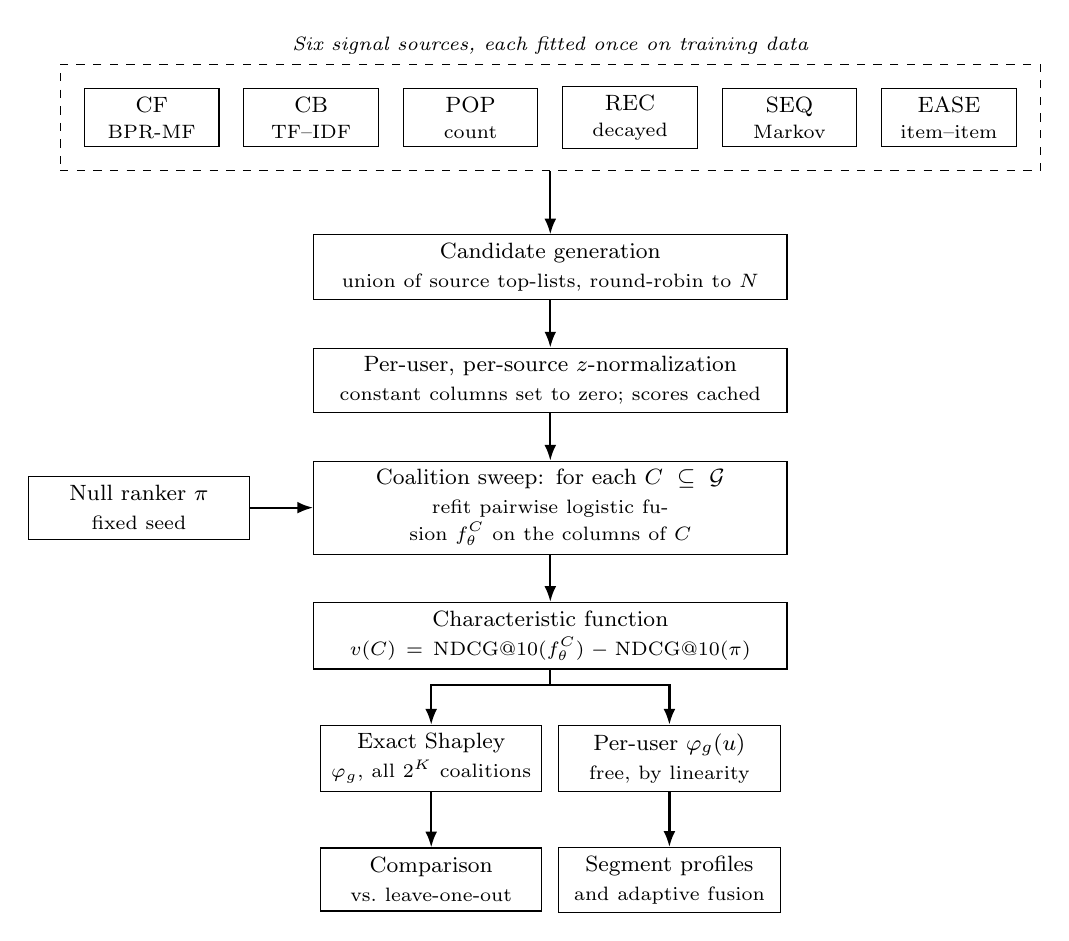
\begin{tikzpicture}[
  font=\footnotesize,
  node distance=6mm,
  box/.style   = {draw, rectangle, minimum height=8mm, align=center,
                  inner xsep=3pt, inner ysep=3pt},
  wide/.style  = {box, text width=58mm},
  narrow/.style= {box, text width=26mm},
  src/.style   = {box, text width=15mm, minimum height=7mm},
  grp/.style   = {draw, dashed, inner sep=3mm},
  ar/.style    = {-{Latex[length=2mm]}, thick},
]

%% --- the six signal sources, trained once ---
\node[src] (cf)   {CF\\\scriptsize BPR-MF};
\node[src, right=3mm of cf]   (cb)   {CB\\\scriptsize TF--IDF};
\node[src, right=3mm of cb]   (pop)  {POP\\\scriptsize count};
\node[src, right=3mm of pop]  (rec)  {REC\\\scriptsize decayed};
\node[src, right=3mm of rec]  (seq)  {SEQ\\\scriptsize Markov};
\node[src, right=3mm of seq]  (ease) {EASE\\\scriptsize item--item};

\node[grp, fit=(cf)(ease),
      label={[font=\scriptsize\itshape]above:Six signal sources, each fitted once on training data}]
      (srcgrp) {};

%% --- candidate generation ---
\node[wide, below=8mm of srcgrp] (cand)
  {Candidate generation\\[1pt]
   \scriptsize union of source top-lists, round-robin to $N$};

%% --- normalization + caching ---
\node[wide, below=6mm of cand] (norm)
  {Per-user, per-source $z$-normalization\\[1pt]
   \scriptsize constant columns set to zero; scores cached};

%% --- coalition sweep (the only repeated step) ---
\node[wide, below=6mm of norm] (fuse)
  {Coalition sweep: for each $C\subseteq\mathcal{G}$\\[1pt]
   \scriptsize refit pairwise logistic fusion $f_\theta^{C}$ on the columns of $C$};

\node[narrow, left=8mm of fuse] (null)
  {Null ranker $\pi$\\[1pt]\scriptsize fixed seed};

\node[wide, below=6mm of fuse] (value)
  {Characteristic function\\[1pt]
   \scriptsize $v(C)=\mathrm{NDCG@10}(f_\theta^{C})-\mathrm{NDCG@10}(\pi)$};

%% --- attribution ---
\node[narrow, below left=7mm and 1mm of value.south] (shap)
  {Exact Shapley\\[1pt]\scriptsize $\varphi_g$, all $2^{K}$ coalitions};
\node[narrow, below right=7mm and 1mm of value.south] (peruser)
  {Per-user $\varphi_g(u)$\\[1pt]\scriptsize free, by linearity};

\node[narrow, below=7mm of shap] (loo)
  {Comparison\\[1pt]\scriptsize vs.\ leave-one-out};
\node[narrow, below=7mm of peruser] (seg)
  {Segment profiles\\[1pt]\scriptsize and adaptive fusion};

%% --- arrows ---
\draw[ar] (srcgrp.south) -- (cand.north);
\draw[ar] (cand)  -- (norm);
\draw[ar] (norm)  -- (fuse);
\draw[ar] (fuse)  -- (value);
\draw[ar] (null.east) -- (fuse.west);
\draw[ar] (value.south) -- ++(0,-2mm) -| (shap.north);
\draw[ar] (value.south) -- ++(0,-2mm) -| (peruser.north);
\draw[ar] (shap)    -- (loo);
\draw[ar] (peruser) -- (seg);
\end{tikzpicture}
\caption{Workflow of the proposed framework. The six signal sources are
fitted once; only the fusion layer is refitted per coalition, which is what
makes the exact game affordable. The null ranker $\pi$ defines the zero point
of the characteristic function, and per-user attribution falls out of the same
sweep by linearity.}\label{fig1}
\end{figure}

\subsection{RQ1: exact source attribution}\label{subsec4_3}

Table~\ref{tab4} reports the Shapley value and normalized share of each source on both datasets, with the efficiency identity of Proposition~\ref{prop1} verified numerically; Figure~\ref{fig2} shows the same shares graphically. That final row is a correctness audit and costs nothing to include.

\begin{table}[t]
\caption{Source Shapley values and normalized shares across the three
benchmarks, reported as the \textbf{mean over five seeds} so that this table,
the seed-stability table (Table~\ref{tab11}) and the bootstrap intervals
(Table~\ref{tab15}) all describe the same quantity. $v(\Gset)$ is likewise the
five-seed mean, so the efficiency row verifies Proposition~\ref{prop1} on the
same basis: the allocation sums to the grand-coalition uplift to machine
precision. Values are shown to six decimals. On Amazon-Beauty and
Amazon-Grocery the six displayed per-source values sum to one unit in the last
place above the displayed $v(\Gset)$, because each is rounded independently
before being added; this is display rounding and not a failure of efficiency,
which is verified to $10^{-17}$ on the unrounded values and reported as exactly
zero in the efficiency row.}\label{tab4}
\small
\setlength{\tabcolsep}{4pt}
\begin{tabular}{@{}lcccccc@{}}
\toprule
& \multicolumn{2}{c}{MovieLens-1M} & \multicolumn{2}{c}{Amazon-Beauty} & \multicolumn{2}{c}{Amazon-Grocery} \\
\cmidrule(lr){2-3}\cmidrule(lr){4-5}\cmidrule(lr){6-7}
Source & $\varphi_g$ & \% & $\varphi_g$ & \% & $\varphi_g$ & \% \\
\midrule
\input{\resdir/tab4_body}
\bottomrule
\end{tabular}
\end{table}

\begin{table}[t]
\caption{Shapley values with 95\% bootstrap confidence intervals (1000
resamples over users). Point estimates are the five-seed means of
Table~\ref{tab4}, so the two tables agree. Because Proposition~\ref{prop3}
makes $\varphi_g$ exactly the mean of the per-user values, resampling users is
a bootstrap of that mean and requires no additional coalition refits. The
interval half-widths measure \emph{user-resampling} variability, estimated on
the reference seed; \emph{training-seed} variability is reported separately in
Table~\ref{tab11}, and the two are distinct sources of uncertainty. \cizerotext, whose share is the
smallest positive allocation on that benchmark.}\label{tab15}
\footnotesize
\setlength{\tabcolsep}{2.5pt}
\begin{tabular}{@{}lcccccc@{}}
\toprule
& \multicolumn{2}{c}{MovieLens-1M} & \multicolumn{2}{c}{Amazon-Beauty} & \multicolumn{2}{c}{Amazon-Grocery} \\
\cmidrule(lr){2-3}\cmidrule(lr){4-5}\cmidrule(lr){6-7}
Source & $\varphi_g$ & CI ($\times10^{-3}$) & $\varphi_g$ & CI ($\times10^{-3}$) & $\varphi_g$ & CI ($\times10^{-3}$) \\
\midrule
\input{\resdir/tab15_body}
\bottomrule
\end{tabular}
\end{table}

\begin{table}[t]
\caption{Allocation restricted to the informative subset, that is, users whose
held-out item reaches the top ten under at least one coalition. Every source
is rescaled by the same factor (the reciprocal of the informative fraction),
so the normalized shares are unchanged from Table~\ref{tab4} to $0.000$
percentage points. Reported on the same five-seed-mean basis as
Table~\ref{tab4}.}\label{tab13}
\small
\setlength{\tabcolsep}{4pt}
\begin{tabular}{@{}lcccccc@{}}
\toprule
& \multicolumn{2}{c}{MovieLens-1M} & \multicolumn{2}{c}{Amazon-Beauty} & \multicolumn{2}{c}{Amazon-Grocery} \\
\cmidrule(lr){2-3}\cmidrule(lr){4-5}\cmidrule(lr){6-7}
Source & $\varphi_g$ & \% & $\varphi_g$ & \% & $\varphi_g$ & \% \\
\midrule
\input{\resdir/tab13_body}
\bottomrule
\end{tabular}
\end{table}


\begin{figure}[t]
\centering
\includegraphics[width=0.95\textwidth]{fig2_shares.png}
\caption{Shapley values $\varphi_g$ per source on the three benchmarks. The collaborative item-item source (EASE) dominates both sparse datasets, whereas the sequential source leads only on the dense one.}\label{fig2}
\end{figure}

Before any allocation is read, one diagnostic bounds every per-user statement
in this paper and we state it here rather than in an appendix. Only \infoMl\%
of evaluation users on MovieLens-1M (\ninfoMl\ of \nevalMl), \infoBt\% on
Beauty and \infoGr\% on Grocery have an attribution vector that is not
identically zero. For the remainder the held-out item never reaches the top
ten under \emph{any} of the 64 coalitions, so $v_u(C)=0$ for every $C$ and the
user contributes nothing. The global values in Table~\ref{tab4} are unaffected,
since those users contribute zero to a mean, but the effective sample behind
any per-user or per-segment claim is the informative subset. We report both
denominators wherever a per-user quantity appears, and we treat segments
rather than individuals as the unit of explanation throughout
(Section~\ref{subsec3_6}).

Table~\ref{tab15} adds 95\% bootstrap confidence intervals to that same allocation, and Table~\ref{tab13} repeats it on the informative subset. The efficiency identity holds to \effMl, \effBt, and \effGr\ on the three datasets, which is machine precision in double arithmetic. This row is a correctness audit rather than a finding, but it is the single most useful assertion in the pipeline: essentially any indexing or coalition-weighting error breaks it.

The substantive result is that \emph{the ordering inverts with density, but not along the axis we had pre-registered}. We expected the collaborative matrix-factorization source to dominate the dense benchmark and content plus popularity to overtake it on the sparse one. What we observe instead is that the sequential source leads on dense MovieLens-1M with \shMlSEQ\% of the uplift, while the item-item collaborative source EASE leads on both sparse benchmarks with \shBtEASE\% and \shGrEASE\%. The two collaborative sources jointly account for \shMlCF\%$+$\shMlEASE\% on MovieLens-1M against \shBtCF\%$+$\shBtEASE\% on Beauty, so collaborative signal as a family becomes \emph{more} important under sparsity, not less. This is the opposite of the conventional expectation, and a direct contradiction of our own registered prediction. We report it as such.

The content source behaves as predicted along the density axis, rising from \shMlCB\% on the dense benchmark to \shBtCB\% on Beauty: metadata carries the load precisely where interaction evidence thins out. Its near-zero share on Grocery (\shGrCB\%) is a data limitation rather than a contradiction, since the only usable content attribute in that distribution is a single category identifier per item. Two Beauty-specific numbers should be read with the ordinal-clock confound of Section~\ref{subsec4_1} in mind. REC's share there is the lowest of any source on any benchmark, which is what one expects of a recency source whose half-life is defined in days when the clock has no days. Its bootstrap interval nonetheless stays above zero; the only interval in Table~\ref{tab15} that covers zero is POP on Amazon-Grocery. SEQ's share on Beauty is correspondingly favoured, since the held-out item is by construction the immediate sequence successor. For those two sources the Grocery column, which has genuine timestamps, is the one to trust.

Two consequences for the reading of this table. First, normalized shares are interpretable as percentages only when all $\varphi_g\ge 0$; the one small negative value, content on Grocery, is reported raw and its share is parenthetical. Second, the popularity and recency sources receive modest but non-zero credit everywhere, which becomes the subject of Section~\ref{subsec4_4}.

\subsection{RQ2: Shapley versus leave-one-out under redundancy}\label{subsec4_4}

Table~\ref{tab5} places the Shapley allocation beside the three ablation-style alternatives, with a redundancy diagnostic, the rank correlation between source score columns, in the final column. All four attribution columns are means over the same five seeds as Table~\ref{tab4}, since every one of them is computed from trained fusion layers and inherits that training noise; per-source dispersion is reported in Table~\ref{tab11} for the Shapley column and, for the allocation as a whole, by the bootstrap intervals of Table~\ref{tab15}.

\begin{table}[t]
\caption{Attribution methods compared on MovieLens-1M, all on the
\textbf{five-seed-mean basis} used by Table~\ref{tab4}, so that $\varphi_g$ and
$v(\Gset)$ agree across the two tables. The redundancy column reports the
largest absolute Spearman correlation between a source's score column and that
of any other source. Leave-one-out assigns the second-strongest collaborative
source a \emph{negative} value while the Shapley allocation gives it
\shMlEASE\% of all uplift.}\label{tab5}
\setlength{\tabcolsep}{4.5pt}
\begin{tabular}{@{}lccccc@{}}
\toprule
Source & $\varphi_g$ & LOO & Fwd.\ sel. & Perm. & Max.\ redund. \\
\midrule
\input{\resdir/tab5_ml1m_body}
\bottomrule
\end{tabular}
\end{table}

The headline quantity is the \emph{efficiency gap}. The Shapley shares sum to $v(\Gset)$ by construction, whereas the leave-one-out values have no reason to, and under redundancy they fall short. Summed leave-one-out recovers only \looshMlc\% of the uplift on MovieLens-1M, \looshBtc\% on Beauty, and \looshGrc\% on Grocery. Put the other way: on Grocery, ablation accounts for barely an eighth of the ranking quality it is supposed to explain. A single line conveys the argument more forcefully than any per-source comparison.

The sharpest individual case is the EASE source on MovieLens-1M. Leave-one-out values it at \looMlEASE, a \emph{negative} figure implying the system would improve if the source were removed, while the Shapley value assigns it \phiMlEASE, or \shMlEASE\% of all uplift. The mechanism is exactly the one Proposition~\ref{prop2} describes: the two collaborative sources are mutually substitutable, so deleting either alone changes little because the other absorbs its role, and ablation therefore reports that neither matters. A practitioner acting on the ablation would decommission a source carrying a sixth of the system's measured value. Figure~\ref{fig3} plots the two allocations against each other.

\begin{figure}[t]
\centering
\includegraphics[width=0.95\textwidth]{fig3_loo_vs_shapley.png}
\caption{Leave-one-out against the Shapley allocation, one point per source. Points below the diagonal are sources whose contribution ablation under-reports; points left of the vertical axis are sources ablation reports as harmful.}\label{fig3}
\end{figure}

We are deliberately careful about what this demonstrates. Real data exhibits approximate rather than perfect redundancy, so the observation is \emph{not} an instance of Proposition~\ref{prop2}, and we do not present it as one. Proposition~\ref{prop2} establishes that the failure mode exists in the idealized case; Table~\ref{tab5} shows the two methods disagreeing on real data in the direction that proposition predicts, with the measured redundancy reported alongside so that the reader can judge how close the empirical situation is to the idealized one. The measured redundancy supports this reading with one important qualification. The popularity and recency sources, which we constructed to be near-substitutes, correlate at $\rho=\poprecMl$ on MovieLens-1M and $\rho=\poprecBt$ on Beauty, but at only $\rho=\poprecGr$ on Grocery. The engineered redundancy we had described as structural turns out to be substantially an artifact of coarse or ordinal time resolution: given genuine day-level timestamps spanning fourteen years, time-decayed and static popularity are markedly different signals. We report this because it weakens a claim we had pre-registered, and because the leave-one-out failure is nonetheless \emph{largest} on Grocery, which shows the phenomenon does not depend on that particular engineered pair.

\subsection{RQ3: segment heterogeneity}\label{subsec4_5}

Table~\ref{tab6} reports source shares within each behavioural segment, together with a permutation test for heterogeneity: segment labels are shuffled, the between-segment variance of the shares is recomputed, and the observed statistic is compared against the resulting null distribution. Figure~\ref{fig4} displays the profiles. We do not plot the correspondence between the two segmentations: as reported below, their agreement is indistinguishable from chance and the claim is withdrawn.

\begin{table}[t]
\caption{Source shares (\%) by behavioural segment on MovieLens-1M, from the coldest to the heaviest activity quartile, with a permutation test for heterogeneity over 2000 label shuffles. Entries marked $\dagger$ are negative, so per Section~\ref{subsec3_4} they are not interpretable as percentage shares; the underlying raw $\varphi_g$ values are the meaningful quantity there.}\label{tab6}
\begin{tabular}{@{}lrcccccc@{}}
\toprule
Segment & $n$ & CF & CB & POP & REC & SEQ & EASE \\
\midrule
\input{\resdir/tab6_ml1m_body}
\bottomrule
\end{tabular}
\end{table}

\begin{figure}[t]
\centering
\includegraphics[width=0.95\textwidth]{fig4_segments.png}
\caption{Shapley values by behavioural segment (activity quartiles) on the three benchmarks.}\label{fig4}
\end{figure}
Heterogeneity is significant on all three benchmarks, decisively on MovieLens-1M ($p=\hetpMl$) and Grocery ($p=\hetpGr$) and marginally on Beauty ($p=\hetpBt$). Applying Holm--Bonferroni across the three tests leaves all three below $0.05$, Beauty at $p_{\mathrm{Holm}}=0.0385$. We nonetheless treat the Beauty result as weak rather than settled: it sits an order of magnitude closer to the threshold than the other two, it is the benchmark whose ordinal clock we have already identified as a confound, and a single additional comparison in the family would push it past $0.05$.

The pre-registered expectation was that cold users would derive their uplift from popularity and content while heavy users relied on collaborative and sequential signals, inverting the global ordering within at least one segment. This is only partially borne out. The sequential source leads in every quartile on MovieLens-1M, so the global ordering does not invert there. What does move, and move sharply, is the collaborative matrix-factorization source, which holds roughly a quarter of the uplift in the three lighter quartiles and collapses to near zero among the heaviest users, where the sequential source absorbs almost all credit. On Beauty the content source behaves as the cold-start narrative predicts, taking its largest share in the coldest quartile and declining monotonically with activity.

One claim from the blueprint must be withdrawn. We had proposed to compare behavioural segments against \emph{attribution} segments obtained by clustering the per-user $\varphi(u)$ vectors, expecting an adjusted Rand index \cite{hubert1985} in the range 0.3--0.6, indicating related but not identical partitions. The measured agreement is \ariMl, \ariBt, and \ariGr: indistinguishable from chance. We drop the claim rather than defend it. The likely cause is stated in Section~\ref{subsec3_6}: with a single held-out item per user, $v_u$ takes one of only about eleven values, and clustering such vectors is close to clustering noise. This is also why we report segment aggregates rather than individual attributions as the unit of explanation.

The informative subset introduced in Section~\ref{subsec4_3} bounds every per-user claim, and it is worth being precise about what it does and does not affect. Because the uninformative users contribute exact zeros rather than noise, restricting the allocation to the informative subset rescales every source by the \emph{same} factor, namely the reciprocal of the informative fraction. We verified this numerically: the per-source ratio between the informative-subset allocation and the full allocation is $\rescMl$ on MovieLens-1M, $\rescBt$ on Beauty and $\rescGr$ on Grocery, identical across all six sources to machine precision, and the normalized shares of Table~\ref{tab4} are therefore unchanged to $0.000$ percentage points. Each ratio is the reciprocal of the corresponding informative fraction in Table~\ref{tab2}, as it must be. The global attribution is consequently robust to this restriction. What the restriction does affect is statistical power: the segment heterogeneity tests below and the per-user clustering are driven by \ninfoMl, \ninfoBt\ and \ninfoGr\ users, out of evaluation sets of \nevalMl, \nevalBt\ and \nevalGr, rather than by the full evaluation sets, and we report significance accordingly. Table~\ref{tab13} gives the informative-subset allocation in full.

\subsection{RQ4: segment-adaptive fusion}\label{subsec4_6}

Table~\ref{tab7} compares uniform fusion, globally tuned fusion, and segment-adaptive fusion, with the shrinkage sweep of Equation~\eqref{eq3} shown in Figure~\ref{fig5}.

\begin{table}[t]
\caption{Recommendation quality for the fusion variants on all three
benchmarks. $\lambda=0$ recovers global fusion exactly, so the baseline is
nested and the comparison is honest. The controlled SASRec reference appears
separately in Table~\ref{tab12}. Note that the values here are absolute
NDCG@10, whereas the Shapley values of Table~\ref{tab4} are uplift over the
null ranker and are further divided among six sources; the two are on
different scales and should not be compared entry by entry. A source's
standalone NDCG@10 exceeding its $\varphi_g$ is therefore expected, not
contradictory. Relative changes quoted in the text and in
Table~\ref{tab8} are computed from unrounded values. Recomputing them from the
four-decimal figures shown here can differ by up to a few tenths of a
percentage point, on Amazon-Beauty by roughly $0.3$ points, so the two
should not be expected to agree exactly.}\label{tab7}
\begin{tabular}{@{}lccc@{}}
\toprule
Variant & NDCG@10 & Recall@20 & MRR \\
\midrule
\input{\resdir/tab7_body}
\bottomrule
\end{tabular}
\end{table}

\begin{figure}[t]
\centering
\includegraphics[width=0.85\textwidth]{fig5_lambda.png}
\caption{Effect of the shrinkage parameter $\lambda$ on NDCG@10. $\lambda=0$ is global fusion; $\lambda=1$ is fully segment-specific weights.}\label{fig5}
\end{figure}

The outcome is mixed and we report it as such. On Grocery, segment-adaptive fusion improves NDCG@10 by \gainGr\% over globally tuned fusion, a gain that is significant under a paired $t$-test over users ($p=\advpGr$) and survives Holm--Bonferroni correction. The sweep is monotone in $\lambda$, which is the shape the mechanism predicts, and the improvement is concentrated in the heaviest quartile. On MovieLens-1M and Beauty the gains are \gainMl\% and \gainBt\%, and neither is significant after correction. Beauty deserves a precise statement rather than a summary: its raw paired $t$-test is $p_t=\advpBt$, marginally below the conventional threshold, but the Holm-adjusted value across the three benchmarks is $0.099$, so we do not claim it. Section~\ref{subsec5_5} and Table~\ref{tab18} show that both null results are underpowered ($\powMl\%$ and $\powBt\%$ achieved power), so they are best read as undetected effects rather than demonstrated absences.

This pattern admits a mechanistic explanation, which we state with an
important caveat about its status: it was constructed \emph{after} observing
which benchmark responded, and is therefore a post-hoc rationalization rather
than a pre-registered prediction. We report it because it is testable, not
because it has been tested. Segment-adaptive weights can only help to the extent
that segment-level source profiles actually depart from the global profile: if
every segment wants the same weights, the shrinkage in Equation~\eqref{eq3}
has nothing to recover. Measuring that departure directly, as the mean total
variation between each segment's normalized share vector and the global
one, gives 0.153 on MovieLens-1M, 0.147 on Beauty and 0.288 on Grocery.
Grocery's segments diverge from the global profile by roughly twice as much as
the other two benchmarks', and Grocery is the only benchmark where adaptive
fusion helps. The intervention succeeds on the one benchmark where this divergence is
largest. With three datasets and one success this is a hypothesis, not a
validated decision rule: a threshold fitted on the same three points that
motivated it would be circular. The honest statement is that segment-adaptive
fusion helped only where segment profiles departed substantially from the
global profile, and that whether divergence \emph{predicts} the gain
out-of-sample remains untested. Testing it requires pre-registering a
threshold and evaluating on held-out benchmarks, which we identify as the
natural next step. One observation does survive independently of the
threshold question: statistical significance of heterogeneity is not
sufficient, since heterogeneity is significant on MovieLens-1M
($p=\hetpMl$) where the intervention does nothing.

The honest summary is therefore that segment-adaptive fusion \emph{can} deliver a substantial gain where segment profiles genuinely differ, and delivers nothing where they do not. That is consistent with the mechanism, but it is a weaker claim than the uniform improvement we had pre-registered, and one positive result across three benchmarks does not establish a general method. We also note that the gain on Grocery is concentrated in the heaviest rather than the coldest segment, which is the opposite of the predicted shape. We report the contradiction rather than reframing around it.

\subsection{Sensitivity, stability, and ablations}\label{subsec4_7}

We report the stability of $\varphi$ across five seeds and NDCG@$k$ for $k\in\{5,10,20,50,100\}$ to confirm that the allocation is not an artifact of the rank cutoff. Because the Shapley computation is exact, the only source of variance in $\varphi$ is base-scorer training; the fusion layer is a convex problem with a deterministic solution and contributes none. Across five seeds the source ordering is identical on every dataset, with per-source standard deviations of at most 0.002 (Table~\ref{tab11}).

The cutoff sweep is informative rather than merely reassuring. On MovieLens-1M the sequential source falls monotonically from 58.0\% of the allocation at $k=5$ to 38.7\% at $k=100$, while EASE rises from 12.0\% to 22.8\%. The sequential advantage is real but concentrated at the very top of the ranking, which is consistent with the informative-subset diagnostic of Section~\ref{subsec4_5} and is worth knowing for a practitioner choosing where to spend engineering effort.

Following the discussion of Remark~\ref{rem1}, we additionally apply a rank-preserving but shape-changing transform to each source's scores and re-run the entire game. We use percentile rank within each user's candidate list, applied uniformly to all six sources. This choice is deliberate: a bare logarithm is undefined for the collaborative source, whose raw scores are embedding inner products and therefore unbounded reals, and would fail silently on exactly the source expected to matter most. Percentile rank is domain-safe for every source and exactly rank-preserving. Figure~\ref{fig6} shows the coalition value surface from which all of these quantities are derived.

\begin{figure}[t]
\centering
\includegraphics[width=0.95\textwidth]{fig6_coalitions.png}
\caption{Coalition value surface $v(C)$ across all 64 coalitions. The full numerical table appears in Appendix~\ref{secA2}.}\label{fig6}
\end{figure}

Both invariance checks behave as the theory requires. Under a positive affine rescaling $x\mapsto 3.7x+12.5$ applied to every source, the maximum change in any $\varphi_g$ is \affineShift\ in double precision, which is exact invariance, as Remark~\ref{rem1} states. Under the nonlinear percentile-rank transform the maximum shift is \nonlinShift, which is comparable in magnitude to the smaller Shapley values themselves. This is the outcome the remark explicitly declines to rule out: $z$-normalization cancels location and scale but does not undo a reshaping of the score distribution, and because fusion operates on normalized \emph{values} rather than ranks, the fitted weights and hence $v(C)$ shift. We report the sensitivity rather than claiming a monotone invariance the method does not possess. A practitioner should read the allocation as conditional on the sources reporting scores on their natural scale.

\subsection{Statistical significance}\label{subsec4_8}

Comparisons are paired over \emph{users}, which is the unit of analysis throughout. We report paired $t$-tests with Holm--Bonferroni correction across the method family \cite{holm1979}, Wilcoxon signed-rank tests as a non-parametric companion, and Cohen's $d_z$ as an effect size. Table~\ref{tab8} collects the results.

\begin{table}[t]
\caption{Significance of the segment-adaptive gain over globally tuned fusion,
paired over users, with Holm--Bonferroni correction across the three
benchmarks. $p_t$ is the paired $t$-test, $p_{\mathrm{W}}$ the Wilcoxon
signed-rank test, $p_{\mathrm{Holm}}$ the Holm-adjusted value, and $d_z$
Cohen's effect size for paired samples. By the conventional reading \cite{cohen1988} $|d_z|<0.2$ is negligible, so every effect here is
small in magnitude even where the $p$-value is comfortable: significance is
driven by the number of paired users, not by the size of the per-user
shift.}\label{tab8}
\small
\setlength{\tabcolsep}{4pt}
\begin{tabular}{@{}lcccccc@{}}
\toprule
Dataset & $\Delta$NDCG (\%) & $p_{t}$ & $p_{\mathrm{W}}$ & $p_{\mathrm{Holm}}$ & $d_z$ & Rej. \\
\midrule
\input{\resdir/tab8_body}
\bottomrule
\end{tabular}
\end{table}

\begin{table}[t]
\caption{Stability of the allocation across five random seeds, all three
benchmarks. Because the Shapley computation is exact and the fusion layer is
convex, the only variance source is base-scorer training. CV is the
coefficient of variation (SD/mean, \%); it is large only where the mean is
near zero, notably CB on Grocery.}\label{tab11}
\small
\setlength{\tabcolsep}{3pt}
\begin{tabular}{@{}lccccccccc@{}}
\toprule
& \multicolumn{3}{c}{MovieLens-1M} & \multicolumn{3}{c}{Amazon-Beauty} & \multicolumn{3}{c}{Amazon-Grocery} \\
\cmidrule(lr){2-4}\cmidrule(lr){5-7}\cmidrule(lr){8-10}
Source & Mean & SD & CV & Mean & SD & CV & Mean & SD & CV \\
\midrule
\input{\resdir/tab16_body}
\bottomrule
\end{tabular}
\end{table}


%%%%%%%%%%%%%%%%%%%%%%%%%%%%%%%%%%%%%%%%%%%%%%%%%%%%%%%%%%%%%%%%%%%%%%
\section{Discussion and broader implications}\label{sec5}
%%%%%%%%%%%%%%%%%%%%%%%%%%%%%%%%%%%%%%%%%%%%%%%%%%%%%%%%%%%%%%%%%%%%%%

\subsection{What the attributions mean for system design}\label{subsec5_1}

The practical value of the allocation lies in reading it against the cost column of Table~\ref{tab3}. A source with a small share and a high maintenance cost is a decommissioning candidate, and this is the concrete decision the framework informs, one that ablation cannot inform at all, because ablation may report zero for a source that is in fact load-bearing. The word to stress is \emph{informs}. Because coalitions are scored on a candidate pool built by the full source set, $\varphi_g$ measures what a source contributes at the fusion stage, not what would be lost if it were switched off and stopped feeding retrieval. Appendix~\ref{secA4} bounds the difference empirically: on a matched seed, regenerating candidates per coalition moves no source's share by more than \regenworst\ percentage points and leaves the ordering \regenorder. The allocation is therefore a screening instrument: it identifies which sources are worth the cost of an end-to-end removal trial and, more usefully, which apparent zeros are artifacts of redundancy and should not be cut on the strength of an ablation. Our results supply exactly such a pattern, and it points in a direction we did not anticipate. The sequential source is the most operationally demanding of the six, requiring session logging and low-latency state, and on the dense benchmark it earns that cost, taking \shMlSEQ\% of the uplift. On both sparse benchmarks its share falls to roughly a quarter while the item-item collaborative source, which is a closed-form computation over an interaction matrix with no online state at all, takes \shBtEASE\% and \shGrEASE\%. For a catalogue resembling the sparse benchmarks, the engineering case for maintaining a sequential pipeline is therefore considerably weaker than for maintaining an item-item model, and the allocation quantifies how much weaker.

The contrast with ablation is the practical argument for the method. On MovieLens-1M, leave-one-out reports the EASE source at \looMlEASE, a negative value which a practitioner would read as licence to decommission it, while the Shapley allocation assigns it \shMlEASE\% of the system's measured uplift. Acting on the ablation would remove a load-bearing component, and the reason is precisely the redundancy that Proposition~\ref{prop2} isolates.

\subsection{Cold start as an attribution phenomenon}\label{subsec5_2}

The segment analysis suggests a reframing of cold start. It is conventionally described as a data problem: a new user has too little history for personalization to work. The segment-level allocation describes it instead as a \emph{shift in which source carries the load}, and measures that shift directly. On this reading, a system does not fail for cold users so much as fall back onto a different subset of its own machinery, and the design question becomes which fallback sources deserve investment rather than how to acquire more data.

\subsection{Relation to feature-level explanation}\label{subsec5_3}

Source attribution and feature attribution answer different questions and compose naturally. Once a source has been identified as load-bearing, feature-level attribution \emph{inside} that source is the natural next level of zoom, and this is precisely where the authors' prior clustering-plus-Shapley work \cite{louhichi2023,louhichi2025} fits as the complementary layer. Similarly, the temporal axis of explanation stability is orthogonal to the population axis studied here, and the two could in principle be combined into a source attribution tracked over a stream.

\subsection{Limitations and threats to validity}\label{subsec5_4}

Several limitations should be stated plainly, and a few of them are consequential enough that we would rather raise them than have a reader discover them.

\textbf{The comparison is now controlled, but it is two architectures.}
Section~\ref{subsec4_2} trains SASRec inside our own pipeline on identical
splits and candidate sets, which removes the cross-paper comparability problem
that an earlier version of this work was rightly criticized for. The same protocol is applied to LightGCN \cite{he2020}, so the comparison now spans a sequential and a graph-convolutional reference rather than one architecture. It remains two: we do not claim the hybrid is competitive with every modern sequential, graph-based or generative recommender, only with two standard ones under a matched protocol. LightGCN is trained at its published default configuration with no architecture or schedule search, which likely understates its ceiling; we chose not to search it because selecting the setting that least flatters a competitor would invalidate the comparison it exists to provide.

\textbf{Most users contribute nothing.} Only \infoMl\%, \infoBt\% and \infoGr\% of evaluation users have a non-zero attribution vector (Section~\ref{subsec4_5}). Global values are unaffected, but every per-user and per-segment statement rests on that subset, and a protocol with more than one held-out item per user would give a far less coarse per-user signal.

\textbf{Pre-registered predictions that failed.} We had registered that the collaborative source would dominate the dense benchmark, that attribution segments would partially agree with behavioural segments, that segment-adaptive fusion would improve all benchmarks by 1--3\%, and that the popularity--recency redundancy was structural. The first was contradicted, the second withdrawn, the third held on one benchmark of three, and the fourth proved partly an artifact of time resolution. These are reported in the body rather than revised after the fact.

\textbf{Design and scope.} Score-level fusion is one hybridization pattern among several, and the method does not transfer unchanged to feature-combination or cascade designs, where the coalition structure is constrained rather than free; the Myerson value is the natural tool there. Masking a source at fusion time is not equivalent to never having built it, since the candidate set is generated once from the grand coalition. Offline ranking quality is a proxy for deployed value, and the segment-adaptive gain in particular warrants online validation. Six sources is a design choice, and the exactness argument degrades for a system with thirty, at which point structured approximations become necessary. The allocation is invariant to affine rescaling of a source's scores but not to nonlinear reshaping, as quantified in Section~\ref{subsec4_7}. Amazon-Beauty lacks wall-clock timestamps in the distribution available to us, which handicaps the recency source and advantages the sequential one; Amazon-Grocery was added precisely to control for this, but the Beauty numbers should be read with it in mind. Finally, three datasets, however deliberately contrasted, are three datasets.

%%%%%%%%%%%%%%%%%%%%%%%%%%%%%%%%%%%%%%%%%%%%%%%%%%%%%%%%%%%%%%%%%%%%%%
\subsection{Threats to validity}\label{subsec5_5}

We separate threats by the standard four-way taxonomy, since several of them
bound different claims.

\paragraph{Construct validity.}
The attributed quantity is ranking-quality uplift under a fixed retrieval
pool, not the end-to-end value of operating a source. Masking a source at
fusion time leaves the candidate set, which that source helped build,
untouched, so $\varphi_g$ should be read as \emph{fusion-stage credit given a
fixed candidate pool}. This is adequate for setting fusion weights and for ranking sources by marginal ranking power, and it is weaker than what a decommissioning decision strictly requires. Appendix~\ref{secA4} quantifies the gap rather than leaving it as a caveat: on a matched seed, per-coalition candidate regeneration shifts the allocation by at most \regenworst\ percentage points and the source ordering is \regenorder, so the threat is real but small at this catalogue size. Separately, offline NDCG@10 on a
leave-one-out protocol is a proxy for deployed value; no online validation is
reported.

\paragraph{Internal validity.}
Three issues bound the per-user results. First, only \infoMl\%, \infoBt\% and
\infoGr\% of evaluation users have a non-zero attribution vector; as shown in
Section~\ref{subsec4_5} this leaves the global allocation and its normalized
shares unchanged, but it reduces the effective sample of every segment-level
test. Second, each user contributes a single held-out item, so $v_u$ takes one
of roughly eleven values and individual attributions are coarse. Third, the
per-user NDCG that feeds the paired tests is zero-inflated, which violates the
normality assumption of the paired $t$-test; we therefore report the
non-parametric Wilcoxon companion alongside every $t$-test and treat the two
together.

\paragraph{External validity.}
Three datasets, one hybridization pattern (score-level fusion), one fusion family (a convex pairwise logistic ranker) and two reference architectures (SASRec and LightGCN), the latter untuned. The exactness argument depends on $K$ being small; at $K=30$ the
$2^{K}$ sweep is no longer affordable and a structured or sampled
approximation would be required, at which point the paper's central
selling point disappears. Amazon-Beauty carries a known temporal confound
(Section~\ref{subsec4_1}).

\paragraph{Statistical-conclusion validity.}
Effect sizes are small even where significance is comfortable: the Grocery
adaptive gain has $d_z=\dzadaptGr$ at $p_t=\advpGr$, so the result is
detectable rather than large. The two null results require more care, and we
now quantify rather than assert them. Table~\ref{tab18} reports the achieved
power of each paired test at its observed effect size. On Grocery the design
is well powered ($\powGr\%$), so the positive result is trustworthy. On Amazon-Beauty power is only $\powBt\%$ and on MovieLens-1M just $\powMl\%$, the latter being simply $\alpha$ because the observed MovieLens-1M effect is exactly zero and a test has no power against an effect of zero size. At these sample sizes the smallest effect detectable with 80\% power is $d_z=\mdeBt$ and $d_z=\mdeMl$ respectively, both far above the effects observed. \textbf{The two null results are therefore underpowered rather than
demonstrated absences}, and should be read as ``no effect detected at this
sample size'', not as evidence that segment-adaptive fusion does nothing on
those benchmarks. Establishing a true null would require either more
evaluation users or a protocol with more held-out items per user.
Holm--Bonferroni is applied within each comparison family rather than across
the full set of hypotheses tested in the paper. Because that choice is a
judgement call, Table~\ref{tab19} reports the stricter alternative: a single
Holm correction over all \nwidetests\ inferential tests in the manuscript.
\nwidesurvive\ of the \nwidetests\ survive it. Every headline claim is among
the survivors, including both sparse-benchmark comparisons against SASRec, the
MovieLens-1M comparison against LightGCN, segment heterogeneity on
MovieLens-1M and Grocery, and the Grocery adaptive-fusion gain. Two results
that pass their within-family correction do not pass the paper-wide one: the
Grocery comparison against LightGCN ($p_{\mathrm{Holm}}=0.085$) and Beauty
segment heterogeneity ($p_{\mathrm{Holm}}=0.154$). We regard the within-family
correction as the primary analysis, since the four families address unrelated
questions and pooling them is conservative to the point of being
uninformative, but a reader who prefers the strict reading can take
Table~\ref{tab19} at face value: it does not disturb any conclusion the paper
depends on, and it does identify the two results that are threshold
sensitive.

A rank test across datasets was also requested of us, on the grounds that it
would test whether the \emph{ordering} of sources differs by benchmark rather
than only whether individual shares differ from zero. We ran it and report the
outcome, but we do not draw a conclusion from it, because with three datasets
the test is close to powerless by construction. Treating datasets as blocks and
the six sources as treatments, the Friedman statistic is $\chi^{2}_{5}=11.0$
with $p=0.051$. The ceiling matters more than the value: with $N=3$ blocks and
$k=6$ treatments, a \emph{perfectly} concordant ordering, one source ranked
first on every benchmark and another last on every benchmark, attains only
$p=0.010$. The Nemenyi critical difference at $\alpha=0.05$ is $4.35$
average-rank units against a maximum attainable gap of $5.00$, so the post-hoc
test can separate at most the single most extreme pair and in our data
separates none: the largest observed gap is $3.33$ average-rank units, between
SEQ and EASE at $1.67$ and CB and REC at $5.00$. We therefore regard the
cross-dataset ordering claims in Section~\ref{subsec4_3} as descriptive, and
this is a direct consequence of the three-benchmark scope acknowledged in
Section~\ref{subsec5_4} rather than a defect of the test.

\begin{table}[t]
\caption{Paper-wide multiple-comparison audit. A single Holm--Bonferroni
correction is applied across all \nwidetests\ inferential tests in the
manuscript, which is stricter than the within-family correction used in the
primary analysis. Reported so that threshold-sensitive results are visible
rather than obscured by the choice of family.}\label{tab19}
\small
\setlength{\tabcolsep}{4pt}
\begin{tabular}{@{}llccc@{}}
\toprule
Dataset & Test & $p_{t}$ & $p_{\mathrm{Holm}}$ (paper-wide) & Rej. \\
\midrule
\input{\resdir/tab19_body}
\bottomrule
\end{tabular}
\end{table}

\begin{table}[t]
\caption{Achieved power of the paired $t$-tests for segment-adaptive fusion,
computed at the observed effect size with $\alpha=0.05$ (two-sided). MDE is
the smallest $|d_z|$ detectable with 80\% power at the given $n$. Only the
Grocery test is adequately powered; the two null results are underpowered and
are reported as such.}\label{tab18}
\small
\setlength{\tabcolsep}{4pt}
\begin{tabular}{@{}lrccc@{}}
\toprule
Dataset & $n$ & $d_z$ & power & MDE (80\%) \\
\midrule
\input{\resdir/tab18_body}
\bottomrule
\end{tabular}
\end{table}

\section{Conclusion}\label{sec6}
%%%%%%%%%%%%%%%%%%%%%%%%%%%%%%%%%%%%%%%%%%%%%%%%%%%%%%%%%%%%%%%%%%%%%%

We have recast hybrid recommendation as a cooperative game whose players are signal sources rather than features or items, and shown that this single change of player set converts Shapley attribution from an approximation problem into an exact and inexpensive computation. Efficiency yields an additive decomposition of ranking-quality uplift with no residual; leave-one-out, the standard alternative, provably collapses under the redundancy that is endemic to recommendation; and linearity delivers per-user attribution with no further coalition refits, which we aggregate into segment-level source profiles and then exploit to set segment-adaptive fusion weights that improve ranking quality on one of three benchmarks at unchanged inference cost. Empirically, across MovieLens-1M, Amazon-Beauty and Amazon-Grocery the complete 64-coalition game runs in under a minute on a laptop CPU with the efficiency identity holding to machine precision; leave-one-out recovers only \looshMlc\%, \looshBtc\% and \looshGrc\% of the uplift it purports to explain, and in the sharpest case reports a source carrying \shMlEASE\% of the system's value as actively harmful. Attribution is heterogeneous across activity segments on all three benchmarks, decisively on two and marginally on the third, yet converting that heterogeneity into segment-adaptive weights yields a significant \gainGr\% improvement on only one. We also report what did not hold: attribution-derived segments do not correspond to behavioural segments, the engineered popularity--recency redundancy largely disappears once genuine timestamps are available, and the adaptive gain is absent on two benchmarks.

Several directions follow. Replacing z-normalization with per-user percentile-rank normalization would upgrade Remark~\ref{rem1} from affine to full monotone invariance, at the cost of changing what the fusion layer conditions on. A demographic or otherwise privacy-bearing source would make the credit-versus-exposure trade-off the object of study rather than a complication to be avoided. Owen values \cite{owen1977} would apply when sources form a natural hierarchy, such as a collaborative family against a content family, and Myerson values \cite{myerson1977} when the coalition structure is genuinely restricted, as in cascade hybrids where a downstream stage cannot operate without an upstream one. Finally, online or interleaved evaluation would test whether the segment-adaptive gains observed offline survive deployment.

%%%%%%%%%%%%%%%%%%%%%%%%%%%%%%%%%%%%%%%%%%%%%%%%%%%%%%%%%%%%%%%%%%%%%%
\backmatter

\bmhead{Acknowledgements}
The authors thank the anonymous reviewers for their comments.

\section*{Declarations}

\begin{itemize}
\item \textbf{Funding.} The authors declare that no funds, grants, or other support were received during the preparation of this manuscript.
\item \textbf{Competing interests.} The authors declare no competing interests.
\item \textbf{Ethics approval.} Not applicable; the study uses publicly available secondary data with no human participants.
\item \textbf{Consent to participate / for publication.} Not applicable.
\item \textbf{Data availability.} All three benchmarks are derived from public corpora: MovieLens-1M \cite{harper2015}, and the Amazon-Beauty and Amazon-Grocery subsets of the Amazon Reviews corpus \cite{ni2019}.
\item \textbf{Author contributions.} \textbf{M.L.}: conceptualization, methodology, software, formal analysis, investigation, writing, original draft. \textbf{R.N.}: methodology, validation, writing, review and editing. \textbf{M.Lz.}: supervision, conceptualization, writing, review and editing. All authors read and approved the final manuscript.
\end{itemize}

\begin{appendices}

\section{Proofs and notation}\label{secA1}

\noindent\textbf{Proposition~\ref{prop1}.} The Shapley value satisfies efficiency, so $\sum_{g}\varphi_g=v(\Gset)-v(\emptyset)$. By Definition~\ref{def1}, $v(\emptyset)=0$. \hfill$\square$

\medskip
\noindent\textbf{Proposition~\ref{prop2}.} Write $D=\Gset\setminus\{g_1,g_2\}$ and let the redundancy hypothesis $v(C\cup\{g_1\})=v(C\cup\{g_2\})=v(C\cup\{g_1,g_2\})$ hold for every $C\subseteq D$.

\emph{Leave-one-out.} Take $C=D$. Then $\LOO(g_1)=v(\Gset)-v(\Gset\setminus\{g_1\})=v(D\cup\{g_1,g_2\})-v(D\cup\{g_2\})=0$ by the hypothesis, and symmetrically $\LOO(g_2)=0$.

\emph{Symmetry.} For any $C\subseteq D$ the hypothesis gives $v(C\cup\{g_1\})=v(C\cup\{g_2\})$, and for any $C\subseteq D$ we also have $v(C\cup\{g_2\}\cup\{g_1\})=v(C\cup\{g_1\}\cup\{g_2\})$ trivially. Hence $g_1$ and $g_2$ are symmetric players and the symmetry axiom gives $\varphi_{g_1}=\varphi_{g_2}$.

\emph{The common value.} Fix $g_1$ and partition the coalitions $C\subseteq\Gset\setminus\{g_1\}$ by whether they contain $g_2$. If $g_2\in C$, write $C=C'\cup\{g_2\}$ with $C'\subseteq D$; the hypothesis gives $v(C'\cup\{g_2,g_1\})=v(C'\cup\{g_2\})$, so the marginal contribution of $g_1$ is exactly zero and the term drops out. If $g_2\notin C$ then $C\subseteq D$, and the hypothesis gives $v(C\cup\{g_1\})=v(C\cup\{g_1,g_2\})$, so the marginal contribution is $v(C\cup\{g_1,g_2\})-v(C)$. Substituting into Definition~\ref{def2} and keeping the original $K$-player weights leaves exactly the surviving half of the sum,
\[
\varphi_{g_1}=\sum_{C\subseteq D}\frac{|C|!\,(K-|C|-1)!}{K!}\bigl[v(C\cup\{g_1,g_2\})-v(C)\bigr],
\]
which is Equation~\eqref{eq4}; the same argument with the roles exchanged gives the identical expression for $\varphi_{g_2}$, re-deriving the symmetry established above. Strict positivity follows because every weight is positive and, under the hypothesis, each bracket is non-negative whenever $v$ is monotone, with at least one strictly positive by assumption.

\emph{What the proof does not license.} The weighted sum above cannot be collapsed to the single difference $v(\Gset)-v(D)$: doing so would retain only the $C=D$ term and discard every lower-order coalition, which is legitimate only when $D=\emptyset$. Remark~\ref{rem2} gives an explicit three-player counterexample where the collapsed expression overstates the true value by fifty percent. \hfill$\square$

\noindent\textbf{Proposition~\ref{prop3}.} The Shapley operator is linear in the characteristic function: for $v=\sum_k \alpha_k v_k$, the value of player $g$ is $\sum_k \alpha_k \varphi_g[v_k]$. Applying this with $\alpha_u=|\Uset|^{-1}$ gives the claim. \hfill$\square$

\medskip
\noindent\textbf{Remark~\ref{rem1}.} Under $s\mapsto as+b$ with $a>0$, the per-user mean and standard deviation map as $\mu\mapsto a\mu+b$ and $\sigma\mapsto a\sigma$, so the normalized value $(as+b-a\mu-b)/(a\sigma)=(s-\mu)/\sigma$ is unchanged. Every downstream quantity is a function of the normalized values alone. \hfill$\square$

\begin{table}[h]
\caption{Notation.}\label{taba1}
\begin{tabular}{@{}ll@{}}
\toprule
Symbol & Meaning \\
\midrule
$\Uset,\Iset$              & user and item sets \\
$\Gset=\{g_1,\dots,g_K\}$  & signal sources, the players; $K=6$ \\
$s_g(u,i)$                 & score assigned to $(u,i)$ by source $g$ \\
$C\subseteq\Gset$          & a coalition of sources \\
$f_\theta^{C}$             & fusion model refitted on the sources in $C$ \\
$v(C)$, $v_u(C)$           & characteristic function, globally and for user $u$ \\
$\varphi_g$, $\varphi_g(u)$& Shapley value of source $g$, globally and for user $u$ \\
$\bar\varphi_g$            & normalized source share \\
$\mathcal{S}_1,\dots,\mathcal{S}_M$ & user segments \\
$\pi$                      & null ranker, uniform random under a fixed seed \\
$N$                        & candidate-set size per user \\
$A^{\Gset}_u$              & candidate pool for user $u$, built once from $\Gset$ \\
$z_{g,u,i}$                & per-user, per-source $z$-normalized score \\
$P_u$, $R$                 & sampled training pairs for user $u$, and $R=|P_u|$ \\
$\alpha$                   & inverse regularization of the fusion layer \\
$\lambda$                  & shrinkage toward global fusion weights \\
\bottomrule
\end{tabular}
\end{table}

\section{Full coalition values}\label{secA2}

Tables~\ref{tabB1}, \ref{tabB2} and \ref{tabB3} give $v(C)$ for every one of the $2^{6}=64$ coalitions on each benchmark. Reporting the game in full is feasible only because it is exact and small, and we include it so that any reader can recompute the allocation of Table~\ref{tab4} directly from these values.

\begin{table}[t]
\caption{Coalition values $v(C)$, MovieLens-1M. All 64 coalitions.}\label{tabB1}
\footnotesize
\setlength{\tabcolsep}{4pt}
\begin{tabular}{@{}p{0.27\linewidth}r@{\hspace{6pt}}p{0.27\linewidth}r@{}}
\toprule
Coalition & $v(C)$ & Coalition & $v(C)$ \\
\midrule
\input{\resdir/appB_ml1m_body}
\bottomrule
\end{tabular}
\end{table}

\begin{table}[t]
\caption{Coalition values $v(C)$, Amazon-Beauty. All 64 coalitions.}\label{tabB2}
\footnotesize
\setlength{\tabcolsep}{4pt}
\begin{tabular}{@{}p{0.27\linewidth}r@{\hspace{6pt}}p{0.27\linewidth}r@{}}
\toprule
Coalition & $v(C)$ & Coalition & $v(C)$ \\
\midrule
\input{\resdir/appB_beauty_body}
\bottomrule
\end{tabular}
\end{table}

\begin{table}[t]
\caption{Coalition values $v(C)$, Amazon-Grocery. All 64 coalitions.}\label{tabB3}
\footnotesize
\setlength{\tabcolsep}{4pt}
\begin{tabular}{@{}p{0.27\linewidth}r@{\hspace{6pt}}p{0.27\linewidth}r@{}}
\toprule
Coalition & $v(C)$ & Coalition & $v(C)$ \\
\midrule
\input{\resdir/appB_grocery_body}
\bottomrule
\end{tabular}
\end{table}

\section{Hyperparameter grids}\label{secA3}

Selected values are those of Table~\ref{tab10}. The collaborative source uses 64 latent factors with regularization and learning rate both 0.01 over 100 iterations; the content source uses sublinear term frequency with a minimum document frequency of 2; the recency source uses a 30-day half-life, interpreted in ordinal sequence steps on Amazon-Beauty for the reason given in Section~\ref{subsec4_1}; the sequential source uses additive smoothing of 1; and EASE uses $\lambda_{\mathrm{E}}=250$, solved by Cholesky factorization rather than explicit inversion so that the $12{,}101$-item Beauty catalogue fits within the 3\,GB memory budget. The fusion layer samples 10 pairs per training user at $C=1.0$ without an intercept. We verified that the allocation is insensitive to the pair count: raising it from 10 to 200 changes NDCG@10 on MovieLens-1M from 0.0722 to 0.0733, and the fusion objective is convex so the fit is deterministic given the sampling seed.

\section{Candidate-set size and the retrieval ceiling}\label{secA4}

Two design choices around candidate generation deserve their own record.

\paragraph{Why the candidate set is fixed across coalitions.}
Regenerating candidates per coalition changes the retrieval ceiling from
coalition to coalition, which breaks the comparability of $v(C)$ that the game
relies on and makes $v$ non-monotone: a coalition could score worse than a
subset of itself purely because it retrieved a harder candidate pool. We
pre-committed to the fixed-candidate design in Section~\ref{subsec3_3} for
this reason. The cost is stated honestly in Section~\ref{subsec5_4}: masking a
source at fusion time is not the same as never having built it, because every
coalition inherits a pool that the grand coalition helped retrieve.

\paragraph{How much the fixed pool changes the allocation.}
The argument above says why the pool is held fixed; it does not say what that
choice costs. Because the objection is about magnitude rather than principle,
we measured it. Table~\ref{tabD2} recomputes the entire game with candidates
\emph{regenerated} from each coalition's own sources, so that a source excluded
from a coalition no longer helps build the pool that coalition is scored on.
This is the end-to-end quantity the fixed-pool design cannot see, and it costs
roughly $2^{K}/K$ times more scoring work, which is why it is a check rather
than the default protocol.

The two protocols coincide exactly at the grand coalition, as they must, since
the regenerated pool for $\Gset$ \emph{is} the fixed pool; $v(\Gset)$ is
identical to machine precision on all three benchmarks, which is a useful
correctness check on the reimplementation. Away from the grand coalition they
differ, and the retrieval ceiling now moves with the coalition: on
MovieLens-1M it ranges from \regenrecminMl\ for the weakest single source to
\regenrecgrandMl\ at the grand coalition, on Amazon-Beauty from
\regenrecminBt\ to \regenrecgrandBt, and on Amazon-Grocery from
\regenrecminGr\ to \regenrecgrandGr. As anticipated, $v$ is no longer monotone
under this protocol on any of the three datasets.

The effect on the allocation is nonetheless small. Comparing the two protocols
on the same seed, so that only the protocol differs, the largest change in any
source's normalized share is \regenmaxMl\ percentage points on MovieLens-1M,
\regenmaxBt\ on Amazon-Beauty and \regenmaxGr\ on Amazon-Grocery, so no share
moves by more than \regenworst\ points anywhere, and the source ordering is
\regenorder. For scale, this is smaller than the seed-to-seed variation of the
fixed protocol itself, which Table~\ref{tab11} reports at up to about two
percentage points. The largest single movement is EASE on MovieLens-1M, which loses
\regenmaxMl\ points once the other sources must retrieve their own candidates;
this is the direction one expects, since EASE is an item--item model whose
retrieved pool overlaps heavily with the collaborative source it is being
separated from.

We draw a bounded conclusion from this. It does \emph{not} show that
fusion-stage credit equals end-to-end source value, and we do not claim it
does. What it shows is that on these three benchmarks the retrieval-stage
contribution of a source is not large enough to reorder the allocation or to
move any share by more than about one point, so the ranking of sources by
credit, which is what Section~\ref{subsec5_1} actually uses, is robust to the
design choice. A source whose value lies mostly in retrieval rather than in
ranking would break this, and we would expect such a source to exist in a
catalogue far larger than ours.

\begin{table}[t]
\caption{Effect of regenerating candidates per coalition. ``Fixed'' is the
protocol used throughout the paper, in which one pool is built from the grand
coalition and shared; ``Regen.'' rebuilds the pool from each coalition's own
sources. Values are normalized Shapley shares in percent, and $\Delta$ is
given in percentage points. \textbf{Both columns are computed on seed
\regenseed\ alone}, not on the five-seed mean used in Table~\ref{tab4}, because
the regenerated protocol costs roughly $2^{K}/K$ times more scoring work than
the fixed one and a five-seed sweep was not affordable. The ``Fixed'' column
therefore differs from Table~\ref{tab4} by the usual seed-to-seed variation of
up to about two percentage points, which Table~\ref{tab11} quantifies
separately. The comparison that matters here is \emph{within} a row: both
columns share a seed, so $\Delta$ isolates the protocol change. The two
protocols agree exactly at the grand coalition by construction.}\label{tabD2}
\small
\setlength{\tabcolsep}{3pt}
\begin{tabular}{@{}lccccccccc@{}}
\toprule
& \multicolumn{3}{c}{MovieLens-1M} & \multicolumn{3}{c}{Amazon-Beauty}
& \multicolumn{3}{c}{Amazon-Grocery} \\
\cmidrule(lr){2-4}\cmidrule(lr){5-7}\cmidrule(lr){8-10}
Source & Fixed & Regen. & $\Delta$ & Fixed & Regen. & $\Delta$
& Fixed & Regen. & $\Delta$ \\
\midrule
\input{\resdir/tabD2_body}
\bottomrule
\end{tabular}
\end{table}

\paragraph{Why $N$ was raised.}
Table~\ref{tabD1} reports the measured ceiling as a function of $N$. At the
conventional $N=200$ the ceiling is 0.504 on MovieLens-1M and 0.160 on
Amazon-Beauty, meaning that on the sparse benchmark more than four fifths of
users could not be served correctly by \emph{any} coalition. Since NDCG is
bounded above by this quantity, attribution computed at $N=200$ would describe
a system whose behaviour is dominated by retrieval failure rather than by
fusion. We therefore raised $N$ to 1000 on MovieLens-1M and 3000 on both
Amazon benchmarks, the smallest round values that clear a 0.5 ceiling. The
ceiling applies uniformly across coalitions, so this rescales all reported
NDCG values without biasing the allocation between sources.

\begin{table}[t]
\caption{Candidate recall ceiling as a function of the candidate-set size
$N$, measured before any attribution was computed. Bold entries are the
selected operating points and correspond to the final column of
Table~\ref{tab2}; the remaining entries are from the $N$-sweep run at
selection time. Dashes mark values not measured, the sweep having already
cleared the threshold. The non-bold entries were measured during model
selection and are reported as recorded; only the selected operating points
were recomputed for the final run, which is why they carry more
decimals.}\label{tabD1}
\begin{tabular}{@{}lccccc@{}}
\toprule
Dataset & $N=200$ & $N=500$ & $N=1000$ & $N=2000$ & $N=3000$ \\
\midrule
MovieLens-1M   & 0.504 & 0.725 & \textbf{0.8847} & ---   & ---   \\
Amazon-Beauty  & 0.160 & 0.245 & 0.346          & 0.500 & \textbf{0.6050} \\
Amazon-Grocery & 0.167 & ---   & 0.383          & 0.516 & \textbf{0.6368} \\
\bottomrule
\end{tabular}
\end{table}

\section{Per-segment attribution in full}\label{secA5}

Table~\ref{tab6} in the main text gives the per-segment allocation for
MovieLens-1M. Tables~\ref{tabE1} and \ref{tabE2} complete the picture for the
two sparse benchmarks. Segments are activity quartiles fitted on training
users only and applied to held-out users by the frozen segmenter, as described
in Section~\ref{subsec3_7}.

The attribution-based segmentation is deliberately not tabulated. Its
agreement with the behavioural segmentation is indistinguishable from chance
on all three benchmarks (adjusted Rand $=\ariMl$, $\ariBt$, $\ariGr$), so the
claim is withdrawn in Section~\ref{subsec4_5} rather than illustrated here.

\begin{table}[t]
\caption{Source shares (\%) by behavioural segment, Amazon-Beauty. Entries marked $\dagger$ are negative, so per Section~\ref{subsec3_4} they are not interpretable as percentage shares; the underlying raw $\varphi_g$ values are the meaningful quantity there.}\label{tabE1}
\begin{tabular}{@{}lrcccccc@{}}
\toprule
Segment & $n$ & CF & CB & POP & REC & SEQ & EASE \\
\midrule
\input{\resdir/tab6_beauty_body}
\bottomrule
\end{tabular}
\end{table}

\begin{table}[t]
\caption{Source shares (\%) by behavioural segment, Amazon-Grocery. Entries marked $\dagger$ are negative, so per Section~\ref{subsec3_4} they are not interpretable as percentage shares; the underlying raw $\varphi_g$ values are the meaningful quantity there.}\label{tabE2}
\begin{tabular}{@{}lrcccccc@{}}
\toprule
Segment & $n$ & CF & CB & POP & REC & SEQ & EASE \\
\midrule
\input{\resdir/tab6_grocery_body}
\bottomrule
\end{tabular}
\end{table}

\section{Attribution baselines on the sparse benchmarks}\label{secA6}

Table~\ref{tab5} in the main text compares the attribution methods on
MovieLens-1M. Tables~\ref{tabF1} and \ref{tabF2} repeat that comparison on the
two sparse benchmarks, where the leave-one-out shortfall is larger still.

\begin{table}[t]
\caption{Attribution methods compared, Amazon-Beauty, on the five-seed-mean basis used throughout.}\label{tabF1}
\setlength{\tabcolsep}{4.5pt}
\begin{tabular}{@{}lccccc@{}}
\toprule
Source & $\varphi_g$ & LOO & Fwd.\ sel. & Perm. & Max.\ redund. \\
\midrule
\input{\resdir/tab5_beauty_body}
\bottomrule
\end{tabular}
\end{table}

\begin{table}[t]
\caption{Attribution methods compared, Amazon-Grocery, on the five-seed-mean basis used throughout.}\label{tabF2}
\setlength{\tabcolsep}{4.5pt}
\begin{tabular}{@{}lccccc@{}}
\toprule
Source & $\varphi_g$ & LOO & Fwd.\ sel. & Perm. & Max.\ redund. \\
\midrule
\input{\resdir/tab5_grocery_body}
\bottomrule
\end{tabular}
\end{table}

\end{appendices}

\bibliography{signalshap-bibliography}

\end{document}
